\documentclass[13pt,a4paper]{extreport}
\usepackage[utf8]{inputenc}
\usepackage[utf8]{vietnam}
\usepackage{amsmath,amsfonts,amssymb}
\usepackage{times}
\usepackage{type1cm}
\usepackage{graphicx}
\graphicspath{{images/android-studio-setup/}{images/jdk-setup/} {images/genymotion-setup/}}
\usepackage{subfig}
\usepackage[unicode,hidelinks=true]{hyperref}
%\usepackage[unicode]{hyperref}
\usepackage{indentfirst}
\usepackage{array}
\usepackage{listings}
\usepackage{comment}
\usepackage{enumerate}
\usepackage{color}
\usepackage{multirow}
\usepackage{multicol}
\usepackage[left=1in,right=1in,top=1in,bottom=2cm]{geometry}
\usepackage{tikz}
\usetikzlibrary{arrows, decorations.markings, calc, fadings, decorations.pathreplacing, patterns, decorations.pathmorphing, positioning, decorations.shapes}

\tikzset{decorate sep/.style 2 args=
{decorate,decoration={shape backgrounds,shape=circle,shape size=#1,shape sep=#2}}}

\definecolor{tdkgreen}{RGB}{0,100,0}
\definecolor{dkgreen}{rgb}{0,0.6,0}
\definecolor{gray}{rgb}{0.5,0.5,0.5}
\definecolor{mauve}{rgb}{0.58,0,0.82}

\lstset{frame=tb,
  %language=C,
  aboveskip=3mm,
  belowskip=3mm,
  showstringspaces=false,
  columns=flexible,
  basicstyle={\small\ttfamily},
  numbers=left,
  numberstyle=\tiny\color{gray},
  keywordstyle=\color{blue},
  commentstyle=\color{dkgreen},
  stringstyle=\color{mauve},
  breaklines=true,
  captionpos=t,
  breakatwhitespace=true,
  tabsize=2
}

\usepackage{titletoc}% http://ctan.org/pkg/titletoc
\titlecontents*{chapter}% <section-type>
  [0pt]% <left>
  {}% <above-code>
  {\bfseries\chaptername\ \thecontentslabel\quad}% <numbered-entry-format>
  {}% <numberless-entry-format>
  {\bfseries\hfill\contentspage}% <filler-page-format>

\setcounter{tocdepth}{3} % Them subsubsection vao muc luc - http://tex.stackexchange.com/questions/146304/subsubsection-in-a-report-style-document
\setcounter{secnumdepth}{3} % Them subsubsection vao lop report - http://tex.stackexchange.com/questions/42161/numbering-subsubsection-in-report-class
\everymath{\displaystyle}
\renewcommand{\arraystretch}{1.3}
%\renewcommand{baselinestretch}{2.0}
\renewcommand{\lstlistingname}{Ch\IeC {\uhorn }\IeC {\ohorn }ng tr\IeC {\`\i }nh}
\renewcommand{\lstlistlistingname}{Danh s\IeC {\'a}ch ch\IeC {\uhorn }\IeC {\ohorn }ng tr\IeC {\`\i }nh}
%http://tex.stackexchange.com/questions/64839/how-to-change-listing-caption

%%\usepackage{fancyhdr}
%%\pagestyle{fancy}
		%\fancyfoot[LE,RO]{\thepage}
%%\fancyhf{}
		%\rhead{}
%%\lhead{\emph{Đề tài: Tìm hiểu thư viện đồ họa OpenGL và Viết ứng dụng}}
%%\renewcommand{\headrulewidth}{0.75pt}
%%\cfoot{\thepage}

\begin{document}
\pagenumbering{gobble}
\begin{titlepage}
\begin{tikzpicture}[remember picture, overlay]
  \draw[line width = 4pt, tdkgreen] ($(current page.north west) + (.7in,-.5in)$) rectangle ($(current page.south east) + (-.55in,.7in)$);
	\end{tikzpicture}
	\centering
	\newcommand{\HRule}{\rule{.3\linewidth}{0.5mm}}
	%\begin{normalsize}
	\vspace{-1.5cm}
	\begin{center}
{\large \textbf{TRƯỜNG ĐẠI HỌC TÂY ĐÔ\vspace{.2cm}\\KHOA KỸ THUẬT -- CÔNG NGHỆ\\\vspace{1.0cm}}}
	\end{center}
 %\end{normalsize}
	
\includegraphics[width=.55\textwidth]{logo_tdu.jpg}\par\vspace{1.0cm}
	{\LARGE \textbf{NIÊN LUẬN 3} \vspace{.5cm} \\  \textbf{TÌM HIỂU THƯ VIỆN ĐỒ HỌA OPENGL}\par}%VÀ VIẾT ỨNG DỤNG
	\vspace{2cm}
	
	\begin{tabular}{ll}
	{\large \textbf{\textit{Giảng viên hướng dẫn}}} & {\qquad \large \textbf{\textit{Sinh viên thực hiện}}}\vspace{.3cm}\\
	{\large \textit{Nguyễn Chí Cường}} & {\qquad \large \textit{Nguyễn Văn Minh Đạt} \hspace{0.7cm}-- $13D480201006$} \vspace{.2cm}\\
	 & {\qquad \large \textit{Nguyễn Thị Thảo Nhu} \hspace{.8cm}-- $13D480201070$} \vspace{.2cm}\\	
	  & {\qquad \large \textit{Nguyễn Thị Phương Thảo} -- $13D480201092$} \vspace{.2cm}\\
	\end{tabular}
	
	\vfill
	
	
	\vfill
	
% Bottom of the page
	{\large \textbf{Cần Thơ, 2016}\vspace{.5cm}}
\end{titlepage}

%%----------------------------------------------------------------------------------------------------------------------------------%%
%%----------------------------------------------------------------------------------------------------------------------------------%%

\begin{tikzpicture}[remember picture, overlay]
  \draw[line width = 4pt] ($(current page.north west) + (.7in,-.5in)$) rectangle ($(current page.south east) + (-.55in,.7in)$);
	\end{tikzpicture}
	\begin{center}	
	%%\centering
	\newcommand{\HRule}{\rule{.3\linewidth}{0.5mm}}
	%\begin{normalsize}
	\vspace{-1.5cm}
	\begin{center}
{\large \textbf{TRƯỜNG ĐẠI HỌC TÂY ĐÔ\vspace{.2cm}\\KHOA KỸ THUẬT -- CÔNG NGHỆ\\\vspace{1.0cm}}}
	\end{center}
 %\end{normalsize}
	
\includegraphics[width=.55\textwidth]{logo_tdu.jpg}\par\vspace{1.0cm}
	{\LARGE \textbf{NIÊN LUẬN 3} \vspace{.5cm} \\  \textbf{TÌM HIỂU THƯ VIỆN ĐỒ HỌA OPENGL}\par}% VÀ VIẾT ỨNG DỤNG
	\vspace{2cm}
	
	\begin{tabular}{ll}
	{\large \textbf{\textit{Giảng viên hướng dẫn}}} & {\qquad \large \textbf{\textit{Sinh viên thực hiện}}}\vspace{.3cm}\\
	{\large \textit{Nguyễn Chí Cường}} & {\qquad \large \textit{Nguyễn Văn Minh Đạt} \hspace{0.7cm}-- $13D480201006$} \vspace{.2cm}\\
	 & {\qquad \large \textit{Nguyễn Thị Thảo Nhu} \hspace{.8cm}-- $13D480201070$} \vspace{.2cm}\\	
	  & {\qquad \large \textit{Nguyễn Thị Phương Thảo} -- $13D480201092$} \vspace{.2cm}\\
	\end{tabular}
	
	\vfill
	
	
	\vfill
	
% Bottom of the page
	{\large \textbf{Cần Thơ, 2016}\vspace{.5cm}}
\end{center}


\newpage
\begin{center}
	\vspace*{50pt}
	\huge{\textbf{Lời cảm ơn\\}}
	\vspace*{10pt}
\end{center}
	
	Chúng em xin chân thành cảm ơn Thầy đã nhiệt tình hướng dẫn nhóm chúng em trong quá trình thực hiện niên luận. Đây là một đề tài mới và khó đối với chúng em, trong quá trình thực hiện niên luận chúng em đã cố gắng nhưng không tránh khỏi sai sót và gặp hạn chế, nhờ thầy nhận xét cho chúng em để bài niên luận hoàn thiện.\\
	
	Cảm ơn cha mẹ, anh chị và bạn bè đã động viên, giúp đỡ chúng con, chúng em trong quá trình thực hiện niên luận.\\
	
	Chúng em xin chân thành cảm ơn!
	\vspace*{10pt}
	\begin{flushright}
		\text{Cần Thơ, ngày 06 tháng 12 năm 2016}\\ \vspace{.5cm}
Nhóm SVTH
	\end{flushright}

%\begin{comment}
\newpage
\begin{center}
	\vspace*{50pt}
	\huge{\textbf{Nhận xét của Giảng viên	hướng dẫn}}
	\vspace*{10pt}
\end{center}	
	\newcommand{\drawdot}{\draw[densely dotted, line width = 1pt]}
	\begin{center}		
		\begin{tikzpicture}
			\draw (0,0) node {$~$};
			\drawdot (1,-1) -- (15,-1);
			\drawdot (0,-2) -- (15,-2);
			\drawdot (0,-3) -- (15,-3);
			\drawdot (0,-4) -- (15,-4);
			\drawdot (0,-5) -- (15,-5);
			\drawdot (0,-6) -- (15,-6);
			\drawdot (0,-7) -- (15,-7);
			\drawdot (0,-8) -- (15,-8);
			\drawdot (0,-9) -- (15,-9);
			\drawdot (0,-10) -- (15,-10);
			\drawdot (0,-11) -- (15,-11);
			\drawdot (0,-12) -- (15,-12);
			\drawdot (0,-13) -- (15,-13);
			\drawdot (0,-14) -- (15,-14);
		\end{tikzpicture}
	\end{center}

	\vspace*{10pt}
	\begin{flushright}
		\textit{Cần Thơ, ngày \ldots tháng \ldots năm 2016}
	\end{flushright}
%\end{comment}

\newpage 

\pagenumbering{roman}

\tableofcontents

\newpage

\listoffigures

\listoftables

%\lstlistoflistings

%%----------------------------------------------------------------------------------------------------------------------------------%%
%%----------------------------------------------------------------------------------------------------------------------------------%%	
\newpage

\pagenumbering{arabic}
%%-------------------------------------------------------------------------------------------------------------------------------------%%
\chapter{Giới thiệu}
\section{Đặt vấn đề}
	OpenGL -- Open Graphics Library: là một trong những thư viện đồ họa phổ biến, được giới thiệu đầu tiên vào năm 1991, dùng làm tiêu chuẩn kỹ thuật đồ họa với mục đích tạo ra giao diện lập trình ứng dụng đồ họa 2D và 3D, cung cấp khoảng 250 hàm để vẽ các đối tượng phức tạp từ những hàm đơn giản (điểm, đoạn thẳng, đa giác,\ldots).\\
	
	OpenGL được ứng dụng rộng rãi trong các trò chơi điện tử, xây dựng các mô hình trong mô phỏng khoa học và thông tin, được dùng để phát triển trò chơi.\\
	
	OpenGL không những chạy được trên máy tính mà còn được mở rộng sang di động, được dùng phát triển nhiều game 2D, 3D trên các hệ điều hành Android, iOS,\ldots \\
	
	OpenGL ES -- Open Graphics Library for Embedded System: là một phiên bản của OpenGL dành cho các hệ thống nhúng, tiêu biểu là các thiết bị di động. OpenGL ES gọn nhẹ và nhẹ hơn so với OpenGL do OpenGL ES được lược bớt một số thành phần để phù hợp hơn với các thiết bị di động có cấu hình thấp hơn máy tính.\\
	
	Các phiên bản của OpenGL ES hỗ trợ cho hệ điều hành Android như sau:
		\begin{itemize}
			\item OpenGL ES 1.0 và 1.1: hỗ trợ Android từ 1.0 trở lên.
			
			\item OpenGL ES 2.0: hỗ trợ Android 2.2 (API level 8) trở lên.
			
			\item OpenGL ES 3.0: hỗ trợ từ Android 4.3 (API level 18) trở lên.
			
			\item OpenGL ES 3.1: hỗ trợ từ Android 5.0 (API level 21) trở lên.
		\end{itemize}
	
	Trong phạm vi đề tài niên luận, nhóm chúng em tìm hiểu về cách sử dụng thư viện đồ họa OpenGL thông qua thư viện OpenGL ES 2.0, một phiên bản dành cho hệ thống nhúng, tiêu biểu là thiết bị di động sử dụng hệ điều hành Android.
\section{Mục tiêu}
	Trong quá trình thực hiện niên luận về đề tài ``\emph{Tìm hiểu về thư viện đồ họa OpenGL}'', mục tiêu chúng em đề ra để đạt được là:
		\begin{itemize}
			\item Biết được một số lĩnh vực cần đến OpenGL: phát triển game, xây dựng các mô hình mô phỏng,\ldots					
			
			\item Biết cách vẽ một số đối tượng cơ bản với các hàm của OpenGL.
			
			\item Biết cách nhúng mã OpenGL (thông qua OpenGL ES 2.0) vào các ứng dụng Android.
		\end{itemize}
	
\section{Phương pháp thực hiện}
	\begin{itemize}
		\item Nội dung và phương pháp thực hiện niên luận của nhóm được trình bày tóm tắt trong bảng~\ref{Tab:phuong-phap-thuc-hien-nien-luan}.
	\begin{table}[!h]
		\begin{center}
			\begin{tabular}{|c|p{9.5cm}|>{\centering\arraybackslash}p{4.5cm}|} \hline
			\textit{STT} & \centering{\textit{Nhiệm vụ}} & \textit{Công cụ} \\ \hline			
			\multirow{2}{.25cm}{1} & \multirow{2}{9.5cm}{Cài đặt môi trường lập trình OpenGL trên Android} & \href{http://www.oracle.com/technetwork/java/javase/downloads/jdk8-downloads-2133151.html}{JDK}, \href{https://developer.android.com/studio/index.html}{Android Studio}, \href{https://www.genymotion.com}{Genymotion}\\ \hline
			2 & Tìm hiểu lý thuyết về OpenGL ES 2.0 trên Android & \href{https://www.khronos.org/opengles/sdk/docs/man/}{OpenGL ES 2.0}\\ \hline
			\multirow{2}{.25cm}{3} & \multirow{2}{9.5cm}{Thực hành một số lệnh cơ bản của OpenGL ES 2.0 trên Android} & \href{http://www.oracle.com/technetwork/java/javase/downloads/jdk8-downloads-2133151.html}{JDK}, \href{https://developer.android.com/studio/index.html}{Android Studio}, \href{https://www.genymotion.com}{Genymotion}\\ \hline
			4 & Quản lý mã nguồn chương trình với Git & \href{https://git-scm.com/}{Git} và \href{https://github.com/}{GitHub}\\ \hline
			\multirow{2}{.25cm}{5} &  \multirow{2}{9.5cm}{Viết báo cáo hoàn thành niên luận} & \LaTeX{} với \TeX{}Maker và \TeX{}Live\\ \hline
		\end{tabular}
		\end{center}
		\caption{Phương pháp thực hiện niên luận}
		\label{Tab:phuong-phap-thuc-hien-nien-luan}
	\end{table}
	
	\item Toàn bộ mã nguồn của bài báo cáo được đưa lên GitHub với địa chỉ:  
	
	\url{https://github.com/minhdatvnus/nienluan3}

\end{itemize}
%%-------------------------------------------------------------------------------------------------------------------------------------%%
\chapter{Cài đặt môi trường lập trình}
\section{Ngôn ngữ lập trình Java}
	Ngôn ngữ lập trình được sử dụng trong đề tài là ngôn ngữ Java. Một chương trình Java có thể được định nghĩa như là một tập hợp các đối tượng giao tiếp thông qua cách gọi những phương thức. Do đó, yêu cầu cần thiết với lập trình Java là phải biết cách lập trình hướng đối tượng -- Object-Oriented Programming.\\
	
	Khi cài đặt Android Studio, thư viện đồ họa OpenGL ES được tích hợp sẳn trong gói phần mềm, do đó chúng ta cần cài đặt JDK và Android Studio là có thể nhúng mã OpenGL vào các ứng dụng Android. Các ứng dụng trên Android được viết bằng ngôn ngữ lập trình Java.\\
	
	Do phạm vi đề tài, nhóm chúng em không đi sâu vào trình bày về ngôn ngữ lập trình Java. Cú pháp các lệnh của ngôn ngữ Java sẽ được giải thích trong các ví dụ khi sử dụng OpenGL trên Android.\\
	
	Chúng ta có thể biên dịch chương trình viết bằng Java trên website: \href{http://browxy.com/}{browxy.com}.
\section{Các phần mềm cần thiết}
	Cần thực hiện cài đặt các phần mềm sau:
	\begin{itemize}
		\item Phần mềm \href{http://www.oracle.com/technetwork/java/javase/downloads/jdk8-downloads-2133151.html}{JDK}: tạo máy ảo Java, dùng biên dịch mã nguồn viết bằng Java.
		\item Phần mềm \href{https://developer.android.com/studio/index.html}{Android Studio}: công cụ lập trình Android.
		
		\item Phần mềm \href{https://www.genymotion.com/}{Genymotion}: phần mềm giả lập điện thoại trên máy tính.
			
			Trong phần mềm Android Studio cũng có máy ảo nhưng chạy chậm hơn so với máy ảo trong phần mềm Genymotion.		
	\end{itemize}
	
	Các cài đặt các phần mềm trên được trình bày trong các mục \ref{Sec:JDK} -- \ref{Sec:Genymotion}.

\section{Cài đặt JDK}\label{Sec:JDK}
	Thực hiện quá trình cài đặt theo các bước bên dưới:
	\begin{itemize}
		\item \textit{Bước 1:} Tải phần mềm \href{http://www.oracle.com/technetwork/java/javase/downloads/jdk8-downloads-2133151.html}{JDK} về máy.
			\begin{itemize}
				\item Truy cập địa chỉ: \url{http://www.oracle.com/technetwork/java/javase/downloads/jdk8-downloads-2133151.html}, được giao diện như hình~\ref{Fig:setup-JDK-1}, click chọn \verb|Accept License Agreement|.				
					\begin{figure}[!h]
						\vspace{-.5cm}
						\begin{center}
								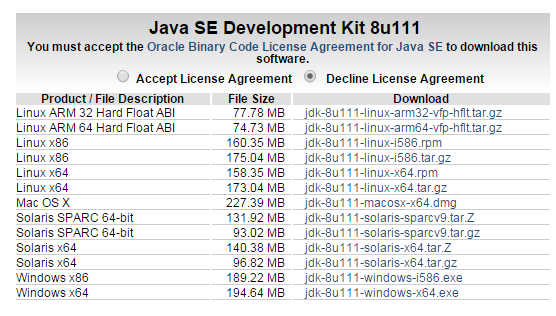
\includegraphics[scale=1]{setup-JDK-1.png}
						\end{center}
						\vspace{-.5cm}
						\caption{Xác nhận đồng ý điều khoản tải JDK về máy}
						\label{Fig:setup-JDK-1}
						\vspace{-.5cm}
					\end{figure}
				
				\item Được giao diện như hình~\ref{Fig:setup-JDK-2}: lựa chọn phiên bản cài đặt phù hợp với hệ điều hành và cấu hình máy để tải về máy. Ví dụ: lựa chọn \verb|Windows x64| ứng với hệ điều hành Windows 64bit.
					\begin{figure}[!h]
						\vspace{-.5cm}
						\begin{center}
							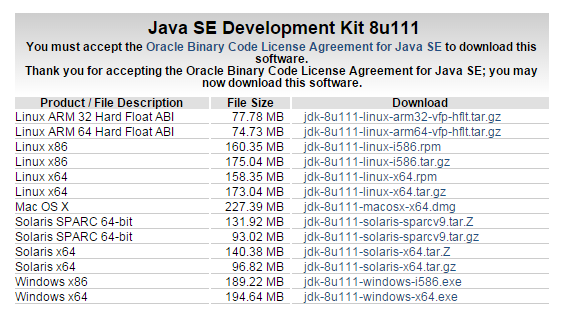
\includegraphics[scale=1]{setup-JDK-2.png}								
						\end{center}
						\caption{Download JDK về máy}
						\label{Fig:setup-JDK-2}
						\vspace{-.5cm}
					\end{figure}
			\end{itemize}

		\item \textit{Bước 2:} Thực hiện cài đặt phần mềm JDK.
			\begin{itemize}
				\item Mở phần mềm JDK vừa tải ở \textit{bước 1}, (ví dụ file \verb|jdk-8u111-windows-x64.exe|) được giao diện như hình~\ref{Fig:setup-JDK-3}. Chọn \verb|Run| để bắt đầu cài đặt JDK.
					\begin{figure}[!h]
						\vspace{-.25cm}
						\begin{center}
							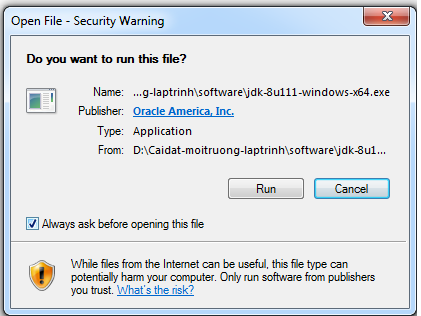
\includegraphics[scale=.65]{setup-JDK-3.png}
						\end{center}
						\vspace{-.25cm}
						\caption{Mở file jdk-8u111-windows-x64.exe để cài đặt JDK}
						\label{Fig:setup-JDK-3}
						\vspace{-.25cm}				
					\end{figure}

				\item Được giao diện như hình~\ref{Fig:setup-JDK-4}: chọn \verb|Next|.
				
				\item Được giao diện như hình~\ref{Fig:setup-JDK-5}: để như mặc định và chọn \verb|Next|.
				
				\item Đợi quá trình cài đặt (hình~\ref{Fig:setup-JDK-6}) hoàn thành như hình~\ref{Fig:setup-JDK-7}: chọn \verb|Close|.		
					\begin{figure}[!h]
						\begin{center}
							\subfloat[Chọn Next\label{Fig:setup-JDK-4}]
								{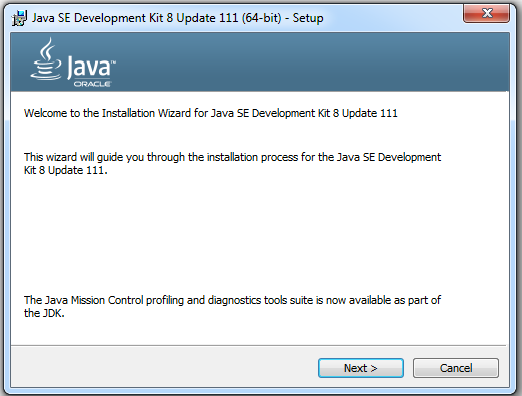
\includegraphics[scale=.5]{setup-JDK-4.png}}
								\hspace{.5cm}
							\subfloat[Chọn Next\label{Fig:setup-JDK-5}]
								{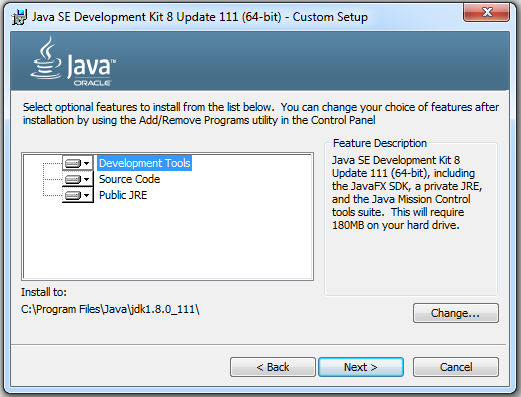
\includegraphics[scale=.5]{setup-JDK-5.png}}\\
							\subfloat[Quá trình cài đặt\label{Fig:setup-JDK-6}]
								{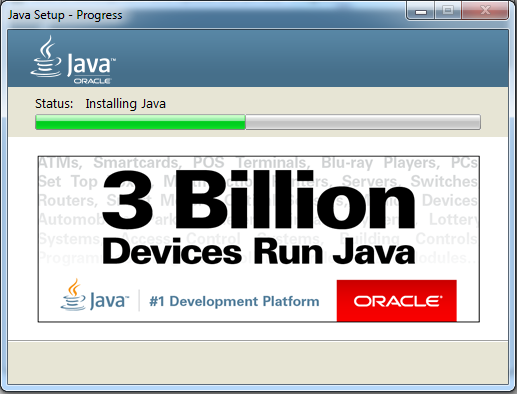
\includegraphics[scale=.5]{setup-JDK-6.png}}
								\hspace{.5cm}
							\subfloat[Chọn Close\label{Fig:setup-JDK-7}]
								{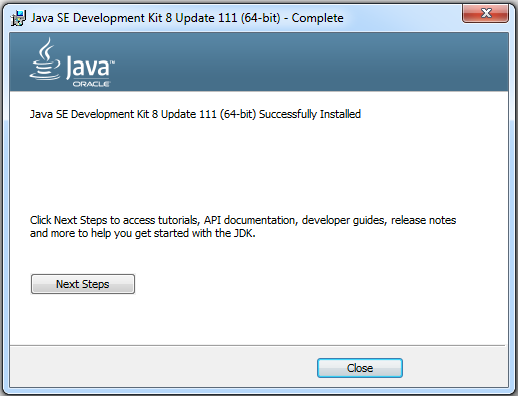
\includegraphics[scale=.5]{setup-JDK-7.png}}								
						\end{center}
						\vspace{-.25cm}
						\caption{Cài đặt JDK trên hệ điều hành Windows}
						\vspace{-.5cm}
					\end{figure}
			\end{itemize}

\newpage			
		\item \textit{Bước 3:} Thiết lập giá trị cho biến \verb|JAVA_HOME|.
			\begin{itemize}
				\item Lấy đường dẫn cài đặt JDK: ví dụ đường dẫn là \verb|C:\Program Files\Java| \verb|\jdk1.8.0_111| (lưu ý là đi đến thư mục \verb|jdk1.8.0_111| như hình~\ref{Fig:local-jdk}).
					\begin{figure}[!h]
						\begin{center}
							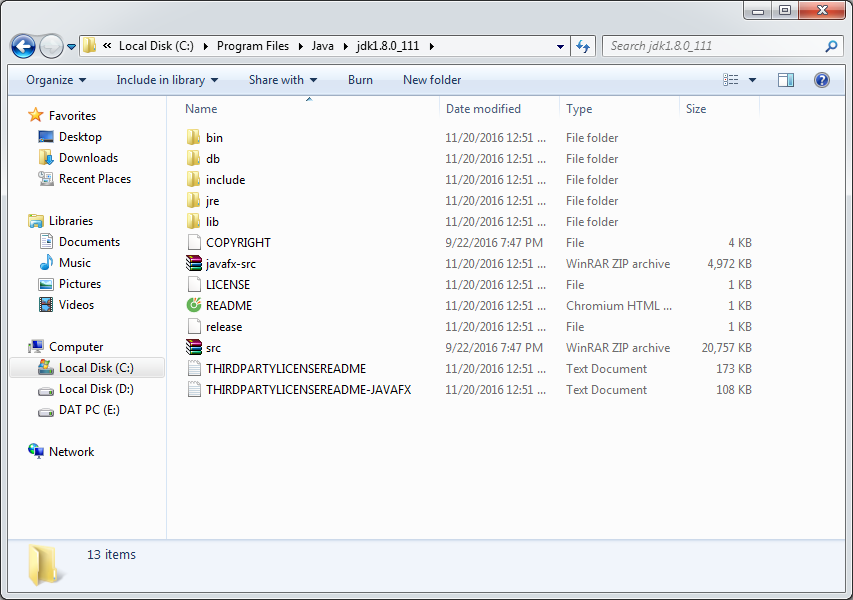
\includegraphics[scale=.5]{local-jdk.png} 
						\end{center}
						\caption{Vị trí của thư mục jdk1.8.0\_111}
						\label{Fig:local-jdk}
					\end{figure}
					
				\item Click chuột phải vào biểu tượng \verb|Computer|, chọn \verb|Properties|, được giao diện như hình \ref{Fig:setup-JDK-JAVA-HOME-1}: chọn \verb|Advanced system settings| bên menu trái.
					\begin{figure}[!h]
						\begin{center}
							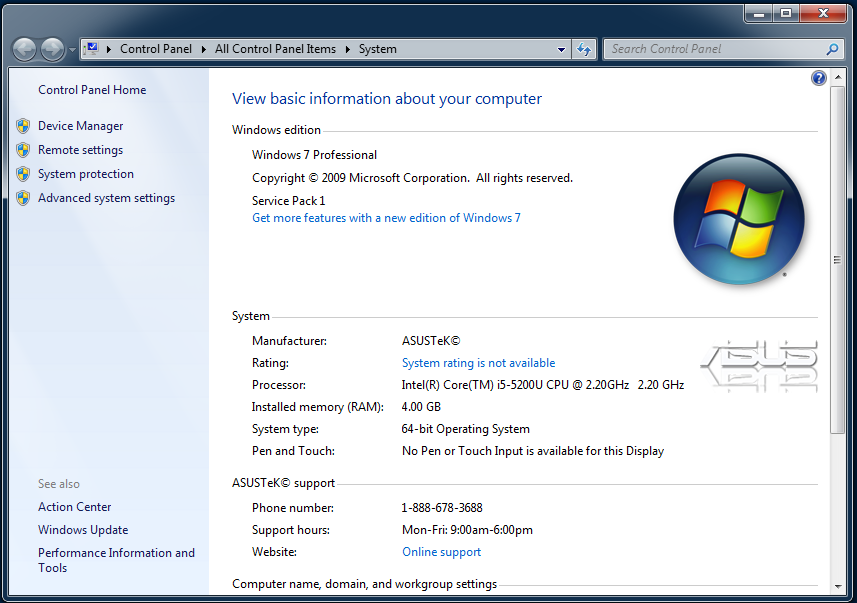
\includegraphics[scale=.5]{setup-JDK-JAVA-HOME-1.png}
						\end{center}
						\caption{Mở của sổ System trên Windows}
						\label{Fig:setup-JDK-JAVA-HOME-1}
					\end{figure}
					
				\item Được cửa sổ như hình~\ref{Fig:setup-JDK-JAVA-HOME-2}: chọn tab \verb|Advanced|, click chọn \verb|Environment| \verb|Variables…| được giao diện như hình~\ref{Fig:setup-JDK-JAVA-HOME-3}.				
					
					\begin{figure}[!h]
						\vspace{-.25cm}
						\begin{center}
							\subfloat[Chọn tab Advanced \label{Fig:setup-JDK-JAVA-HOME-2}]
								{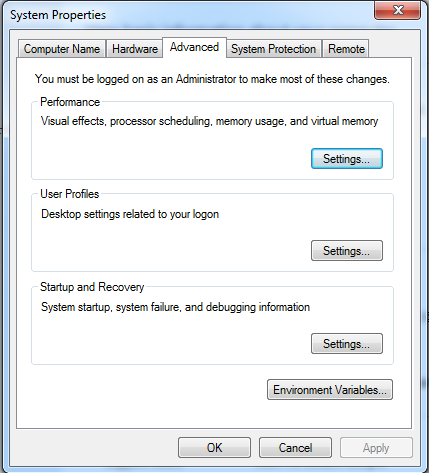
\includegraphics[scale=.6]{setup-JDK-JAVA-HOME-2.png}}
							\hspace{.5cm}
							\subfloat[Cửa sổ Environment Variables…\label{Fig:setup-JDK-JAVA-HOME-3}]
								{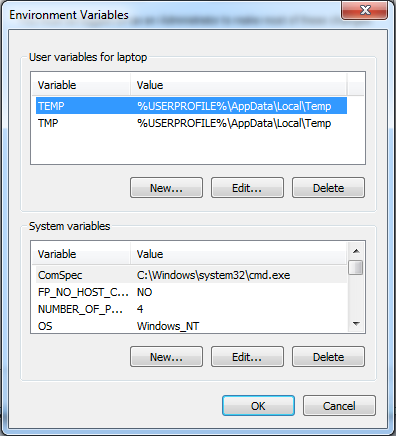
\includegraphics[scale=.65]{setup-JDK-JAVA-HOME-3.png}}\\
							\subfloat[Khởi tạo biến JAVA\_HOME\label{Fig:setup-JDK-JAVA-HOME-4}]
								{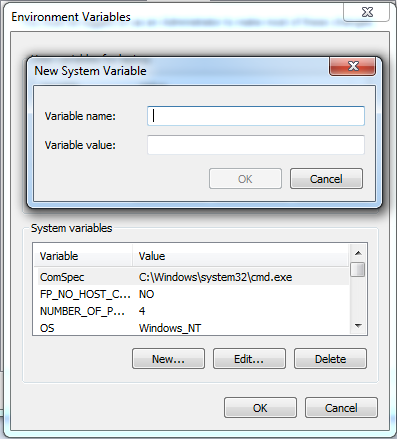
\includegraphics[scale=.65]{setup-JDK-JAVA-HOME-4.png}}
							\hspace{.5cm}
							\subfloat[Giá trị của biên JAVA\_HOME\label{Fig:setup-JDK-JAVA-HOME-5}]
								{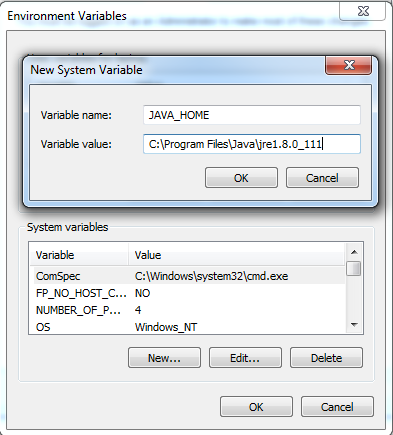
\includegraphics[scale=.65]{setup-JDK-JAVA-HOME-5.png}}
						\end{center}
						\caption{Thiết lập đường dẫn cho biến JAVA\_HOME}
						\label{Fig:setup-JDK-JAVA-HOME}
						\vspace{-.25cm}
					\end{figure}
					
				\item Tìm biến \verb|JAVA_HOME| trong khung \verb|System variables|: nếu có biến \verb|JAVA_HOME| thì không cần thực hiện tiếp. Nếu chưa có biến \verb|JAVA_HOME| thì click chọn \verb|New| để khởi tạo, được giao diện như hình~\ref{Fig:setup-JDK-JAVA-HOME-4}.
				
				\item Trên giao diện hình~\ref{Fig:setup-JDK-JAVA-HOME-4}:
					\begin{list}{+}{}
						\item Ô \verb|Variable Name|: nhập vào \verb|JAVA_HOME|.
						
						\item Ô \verb|Variable value|: nhập vào đường dẫn của thư mục \verb|jdk1.8.0_111| (xác định ở trên), ví dụ: \verb|C:\Program Files\Java\jdk1.8.0_111|
						
						\item Kết quả thiết lập trên hình~\ref{Fig:setup-JDK-JAVA-HOME-5}.
					\end{list}
					
				\item Thực hiện xong chọn \verb|OK|: lúc này biến \verb|JAVA_HOME| đã có trong khung \verb|System variables| (hình~\ref{Fig:setup-JDK-JAVA-HOME-6}). Chọn \verb|OK| để đóng cửa sổ \verb|Environment| \verb|Variables…|, chọn \verb|OK| để đóng cửa số \verb|System Properties|.
					\begin{figure}[!h]
						\begin{center}
							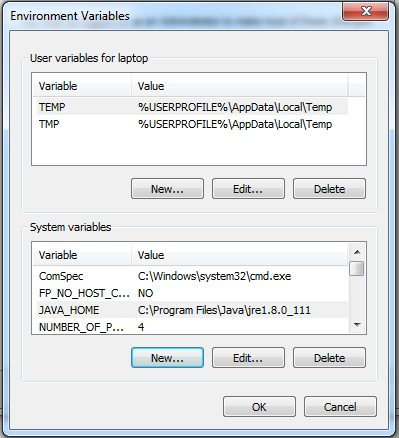
\includegraphics[scale=.65]{setup-JDK-JAVA-HOME-6.png}
						\end{center}
						\caption{Thêm biến JAVA\_HOME vào cửa sổ System variables}
						\label{Fig:setup-JDK-JAVA-HOME-6}
						\vspace{-.5cm}
					\end{figure}
			\end{itemize}
	\end{itemize}
	
\section{Cài đặt Android Studio}\label{Sec:Android}
	Thực hiện quá trình cài đặt theo các bước bên dưới:
	\begin{itemize}
		\item \textit{Bước 1:} Tải phần mềm \href{https://developer.android.com/studio/index.html}{Android Studio} về máy.
			\begin{itemize}
				\item Truy cập vào địa chỉ: \url{https://developer.android.com/studio/index.html}, được giao diện như hình~\ref{Fig:setup-android-1}. Chọn \verb|DOWNLOAD ANDROID| \verb|STUDIO|.				
					\begin{figure}[!h]						
							\begin{center}
								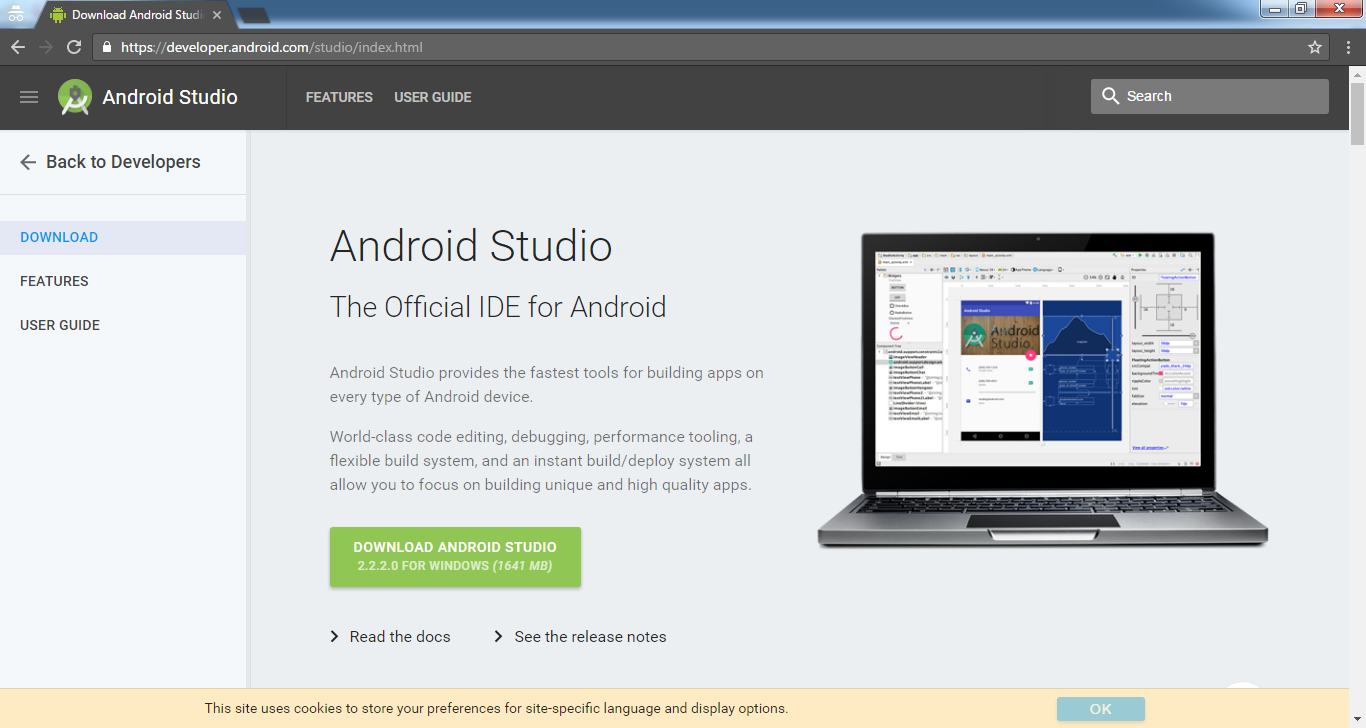
\includegraphics[scale=0.35]{images/android-studio-setup/setup-android-1.png}
							\end{center}
						\caption{Download Android Studio từ trang chủ}
						\label{Fig:setup-android-1}
					\end{figure}

				\item Khi xuất hiện thông báo \verb|Download Android Studio| (trên hình~\ref{Fig:setup-android-2}), check \verb|I have read and argee with the above terms and|
				
				\verb|conditions| để xác nhận đồng ý các điều khoản sử dụng phần mềm.							
					\begin{figure}[!h]
						\begin{center}
							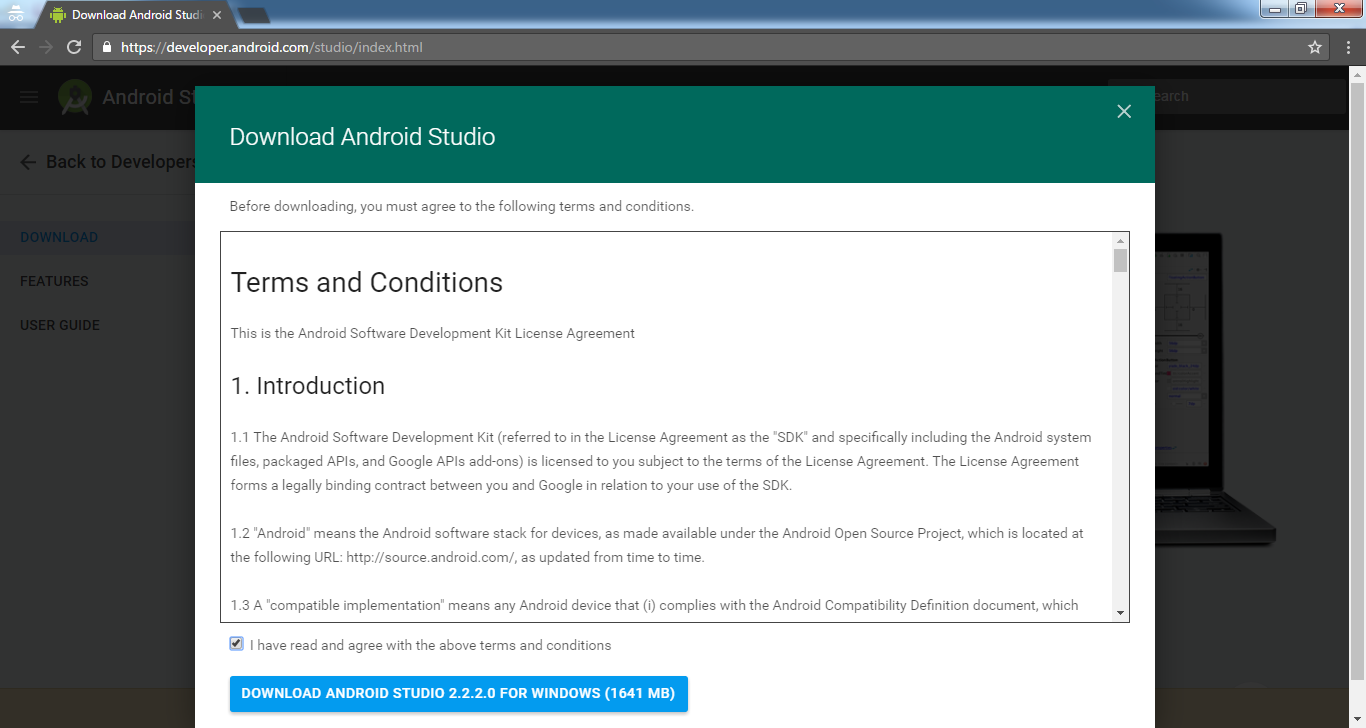
\includegraphics[scale=.35]{setup-android-2.png}						
						\end{center}
						\caption{Xác nhận đồng ý các điều khoản khi Download Android Studio}
						\label{Fig:setup-android-2}
						\vspace{-.25cm}
					\end{figure}
					
				\item Click chọn \verb|DOWNLOAD ANDROID STUDIO 2.2.2.0 FOR WINDOWS| \verb|(1611MB)|, phiên bản hiện tại của Android Studio là 2.2.2.0 và là phiên bản dành cho hệ điều hành Windows.
				
				\item Khi sử dụng Android Studio trên các hệ điều hành khác Windows (ví dụ các bản phân phối Linux,\ldots) thì cách download cũng tương tự (trang web sẽ tự nhận dạng hệ điều hành để đưa phiên bản download hợp lý).
			\end{itemize}

		\item \textit{Bước 2:} Thực hiện cài đặt phần mềm Android Studio.
			\begin{itemize}
				\item Vào ổ đĩa \verb|C| (ổ đĩa hệ thống) tạo thư mục \verb|Android| gồm 2 thư mục con là \verb|Android Studio| và \verb|sdk|.
				
				\item Mở phần mềm \verb|Android Studio| vừa tải về ở \textit{bước 1} (ví dụ tên file là \verb|android-studio-bundle-145.3360264-windows.exe|) được giao diện như hình~\ref{Fig:as-1}. Chọn \verb|Run| để bắt đầu cài đặt \verb|Android Studio|.
					\begin{figure}[!h]
						\begin{center}
							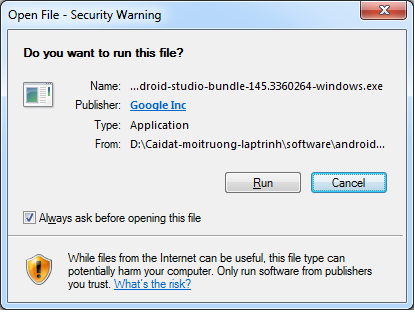
\includegraphics[scale=.65]{as-1.png}
						\end{center}
						\caption{Mở file android-studio-bundle-145.3360264-windows.exe để cài đặt}
						\label{Fig:as-1}
						\vspace{-1cm}
					\end{figure}

\newpage					
				\item Giao diện mới xuất hiện như hình~\ref{Fig:as-2}. Chọn \verb|Next|.
				
				\item Được giao diện như hình~\ref{Fig:as-3}: để như mặc định, chọn \verb|Next|.
				
				\item Được giao diện như hình~\ref{Fig:as-4}: để như mặc định, chọn \verb|I Agree|.	
					
					\begin{figure}[!h]
						\vspace{-.25cm}
						\begin{center}
							\subfloat[Chọn Next\label{Fig:as-2}]
								{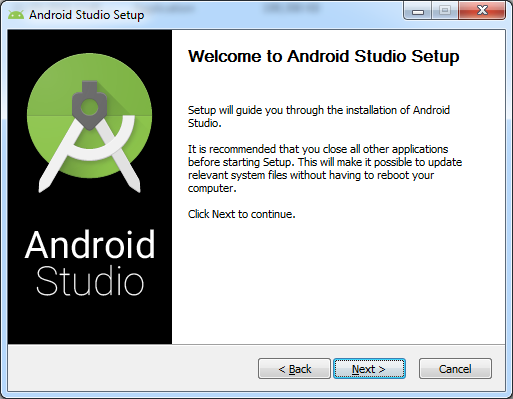
\includegraphics[scale=.5]{as-2.png}}
							\hspace{.5cm}
							\subfloat[Chọn Next\label{Fig:as-3}]
								{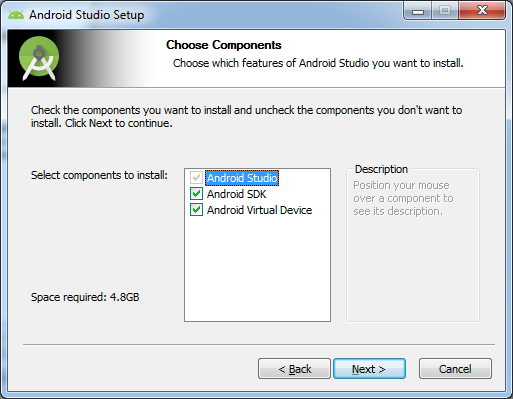
\includegraphics[scale=.5]{as-3.png}}\\
							\subfloat[Chọn I Agree\label{Fig:as-4}]
								{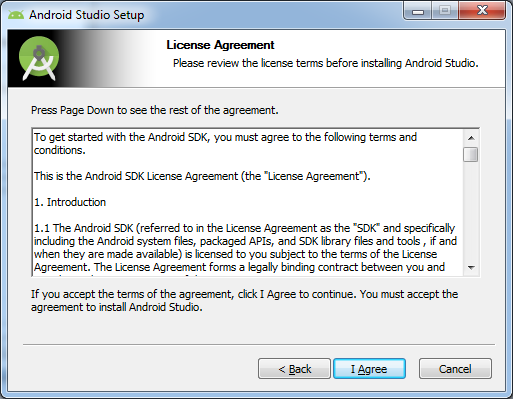
\includegraphics[scale=.5]{as-4.png}}
							\hspace{.5cm}
							\subfloat[Chọn nơi cài đặt Android Studio và SDK \label{Fig:as-5}]
								{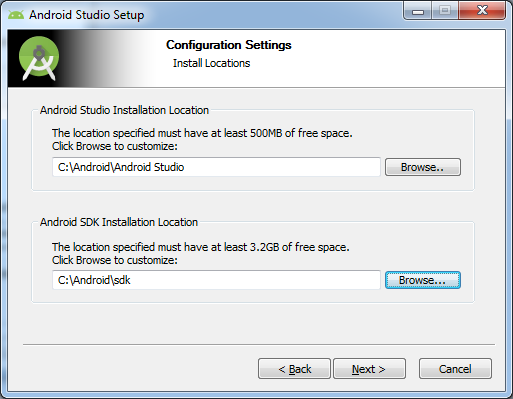
\includegraphics[scale=.5]{as-5.png}}\\
							\subfloat[Chọn Install\label{Fig:as-6}]
								{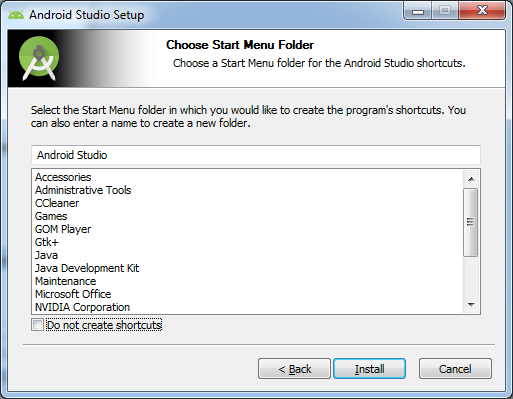
\includegraphics[scale=.5]{as-6.png}}
							\hspace{.5cm}
							\subfloat[Chọn Next\label{Fig:as-7}]
								{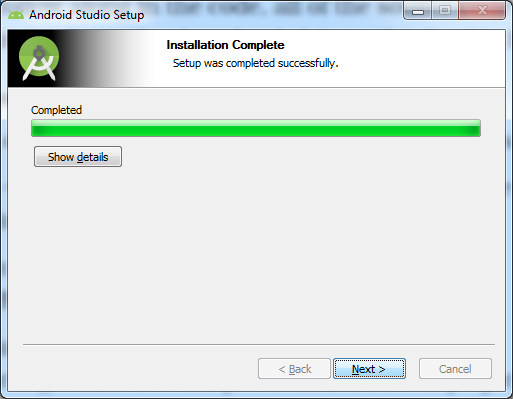
\includegraphics[scale=.5]{as-7.png}}\\
						\end{center}
						\caption{Cài đặt Android Studio trên hệ điều hành Windows}
						\label{Fig:setup-android-studio-window}
						\vspace{-.25cm}
					\end{figure}
					
					\item Được giao diện như hình~\ref{Fig:as-5}: chọn nơi cài đặt vào các thư mục đã được tạo trước đó \verb|Android Studio| và \verb|sdk|.
					\begin{list}{+}{}
						\item Trong khung \verb|Android Studio Installation Location|: dẫn đến thư mục \verb|C:\Android\Android Studio|
						
						\item Trong khung \verb|Android SDK Installation Location|: dẫn đến thư mục \verb|C:\Android\sdk|	
						
						\item Chọn \verb|Next| để sang bước tiếp theo.
					\end{list}
					
				\item Được giao diện như hình~\ref{Fig:as-6}: chọn \verb|Install| để tiến hành cài đặt \verb|Android| 
				
				\verb|Studio| và \verb|Android SDK|.
				
				\item Đợi quá trình cài đặt hoàn thành được giao diện như hình~\ref{Fig:as-7}: Chọn \verb|Next|.
			\end{itemize}
		
		\item \textit{Bước 3:} Cài đặt \verb|Android Studio Wizard|.
			\begin{figure}[!h]
				\vspace{-.6cm}
						\begin{center}
							\subfloat[Chọn OK\label{Fig:as-8}]
								{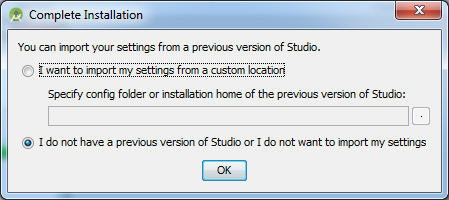
\includegraphics[scale=.63]{as-8.png}}
								\hspace{.5cm}
							\subfloat[Chọn Next\label{Fig:as-9}]
								{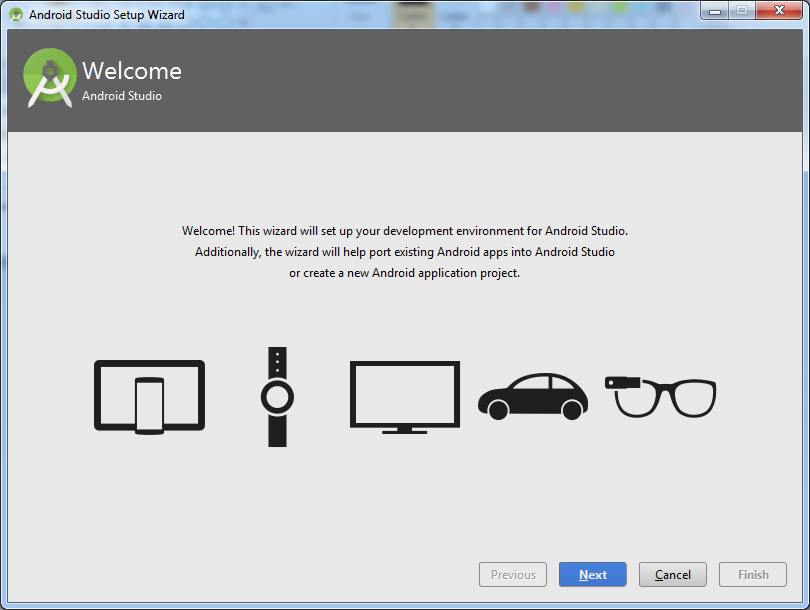
\includegraphics[scale=.35]{as-9.png}}\\
							\subfloat[Chọn Next\label{Fig:as-10}]
								{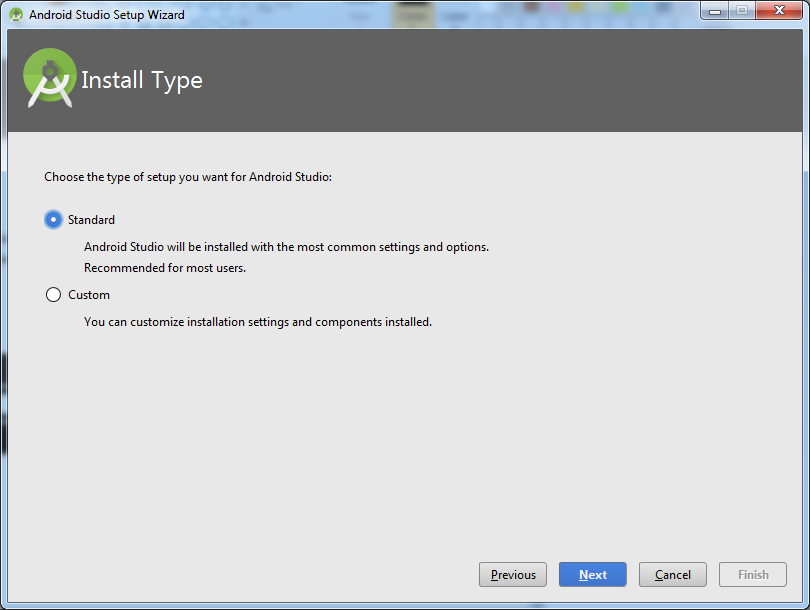
\includegraphics[scale=.35]{as-10.png}}
								\hspace{.5cm}
								\subfloat[Chọn Finish\label{Fig:as-11}]
								{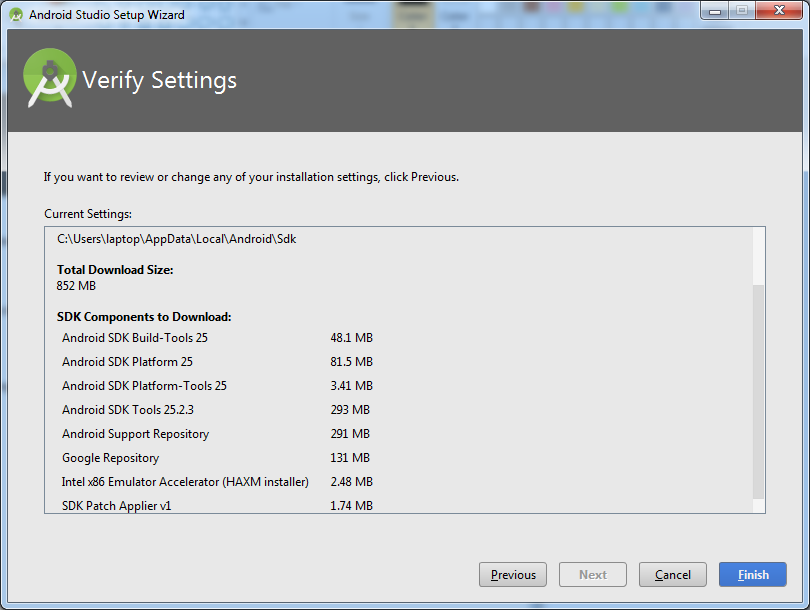
\includegraphics[scale=.35]{as-11.png}}\\
							\subfloat[Chọn Finish\label{Fig:as-12}]
								{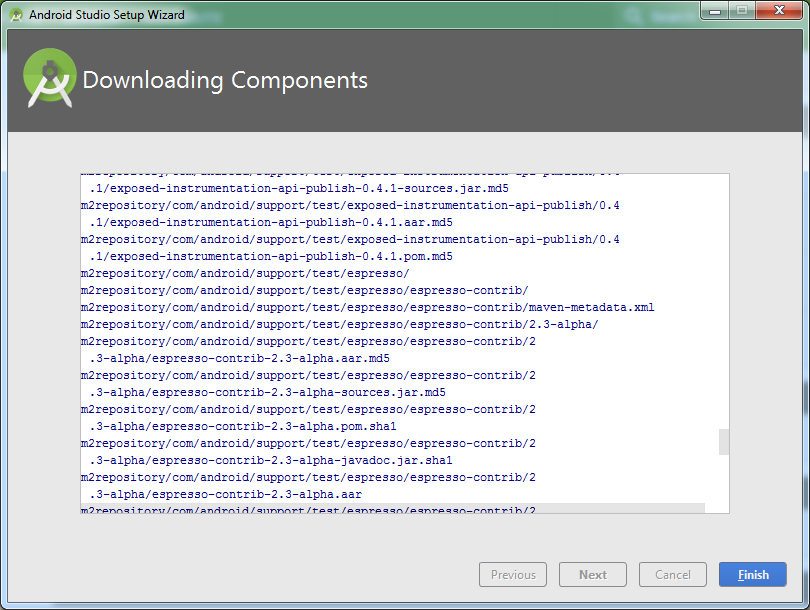
\includegraphics[scale=.35]{as-12.png}}
							\hspace{.5cm}
							\subfloat[Mở Android Studio lần đầu tiên\label{Fig:as-13}]
								{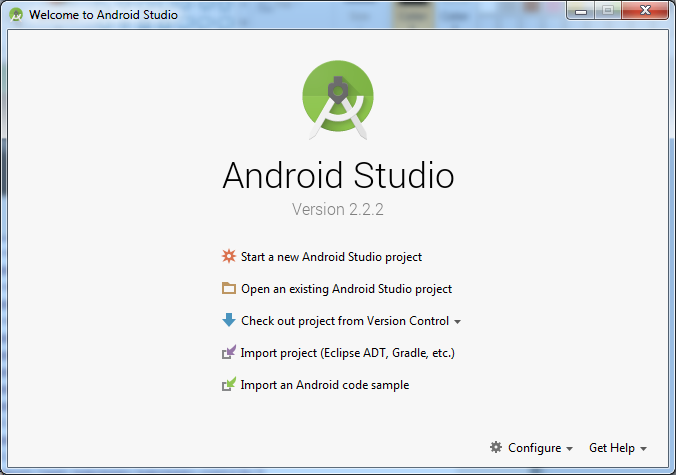
\includegraphics[scale=.43]{as-13.png}}
							
						\end{center}
						\vspace{-.5cm}
						\caption{Cài đặt Android Studio Wizard}
						\label{Fig:setup-android-studio-wizard-window}
						\vspace{-1.25cm}
					\end{figure}
			\begin{itemize}
				\item Sau khi cài đặt \verb|Android Studio| và \verb|Android SDK| xong, xuất hiện thông báo như hình~\ref{Fig:as-8}. Nếu chưa cài đặt phiên bản Android Studio nào trước đó thì chọn \verb|I do not have a previsous version of|
				
				\verb|Studio or I do not want to import my settings| rồi chọn \verb|OK|.
				
				\item Được giao diện như hình~\ref{Fig:as-9}: chọn \verb|Next|.
				
				\item Được giao diện như hình~\ref{Fig:as-10}: để mặc định -- \verb|Standard|, chọn \verb|Next|.
				
				\item Được giao diện như hình \ref{Fig:as-11}: chọn \verb|Finish|.
				
				\item Được giao diện như hình \ref{Fig:as-12}: chọn \verb|Finish|.								
			\end{itemize}

		\item Khi quá trình cài đặt hoàn thành, mở Android Studio lên có giao diện như hình~\ref{Fig:as-13}.	
	\end{itemize}

\section{Cài đặt Genymotion}\label{Sec:Genymotion}
	Thực hiện quá trình cài đặt theo các bước bên dưới:
		\begin{itemize}
			\item \textit{Bước 1:} Tải phần mềm \href{https://www.genymotion.com/}{Genymotion} về máy.
				\begin{itemize}
					\item Truy cập vào địa chỉ \url{https://www.genymotion.com}, được giao diện như hình~\ref{Fig:setup-genymotion-1}, để download phần mềm cần thực hiện đăng nhập (nếu chưa có tài khoản thì tạo mới).
						\begin{figure}[!h]
							\begin{center}
								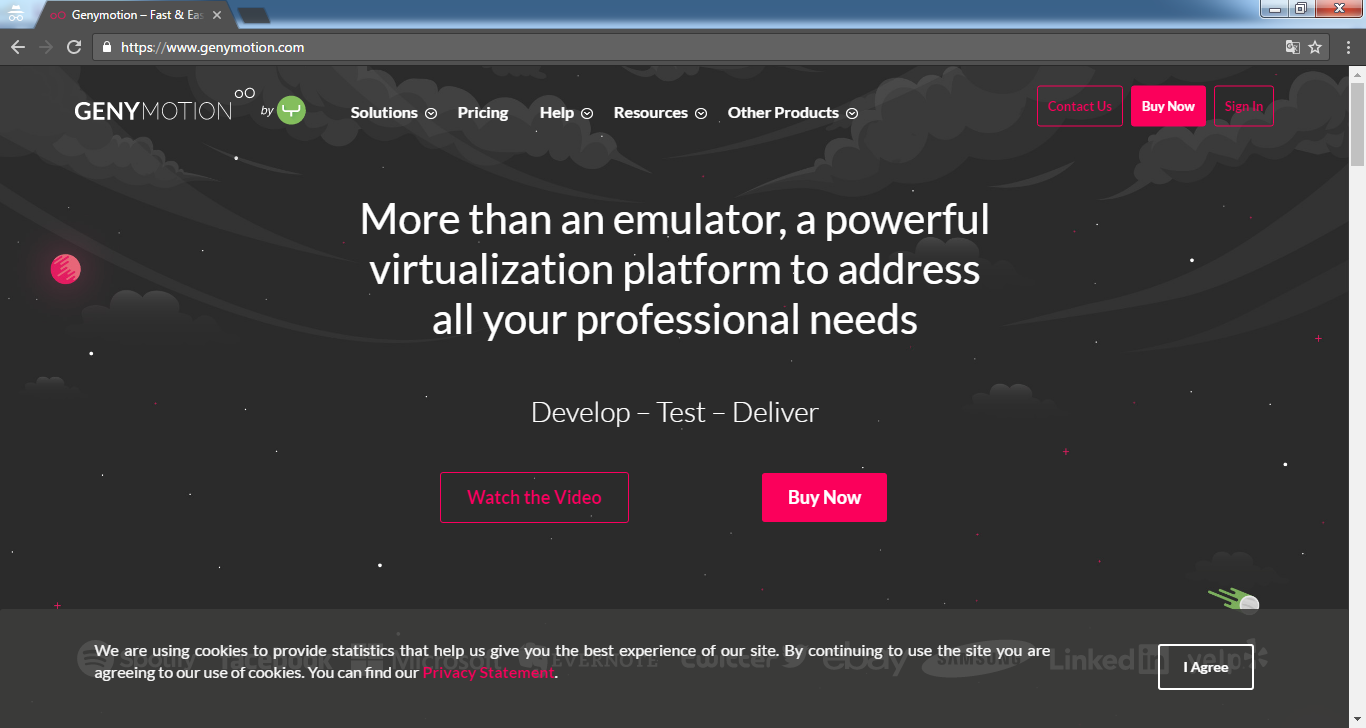
\includegraphics[scale=.35]{setup-genymotion-1}
							\end{center}
							\caption{Trang chủ của Genymotion}
							\label{Fig:setup-genymotion-1}
						\end{figure}
						
					\item Click vào nút \verb|Sign In| được giao diện như hình~\ref{Fig:setup-genymotion-2}, điền thông tin đăng nhập hoặc đăng ký tài khoản mới.
					
					\item Sau khi đăng nhập thành công được giao diện như hình~\ref{Fig:setup-genymotion-3}: click chọn \verb|Get a license|.
						\begin{figure}[!h]
							\begin{center}
								\subfloat[Điền thông tin đăng nhập hoặc đăng ký tài khoản\label{Fig:setup-genymotion-2}]
									{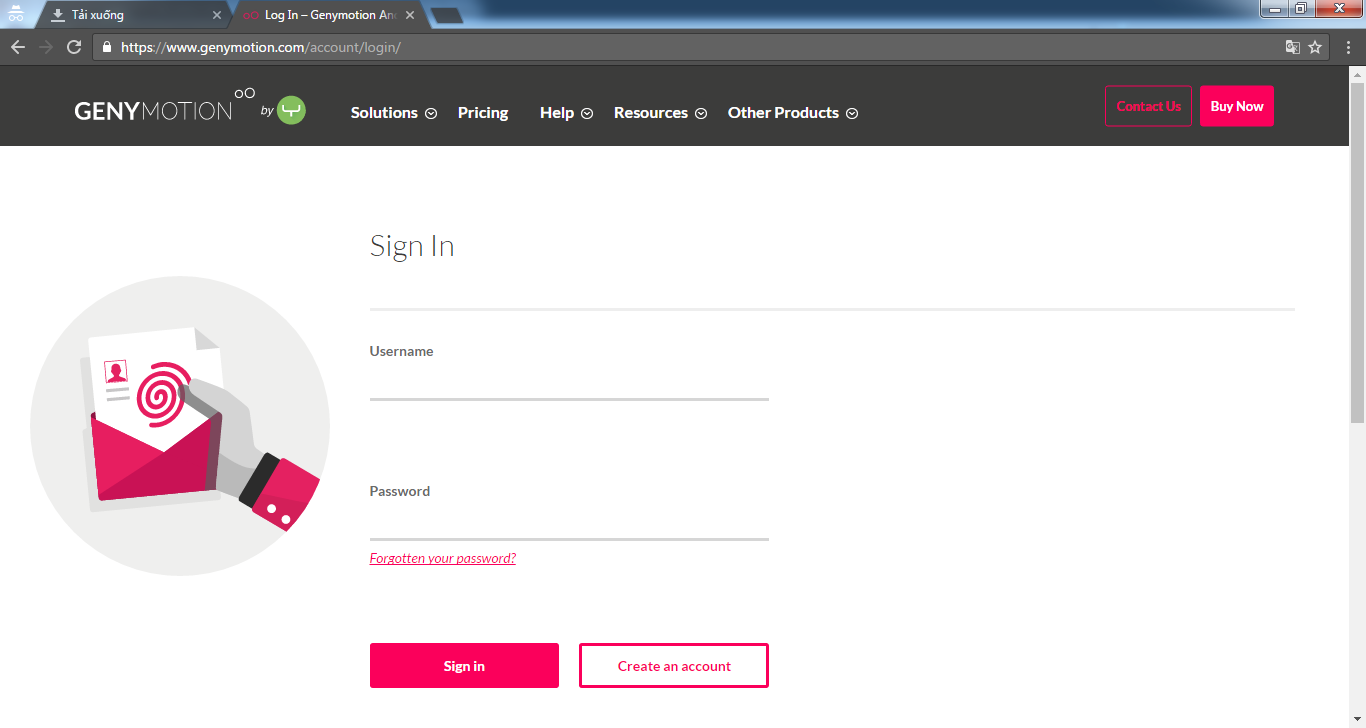
\includegraphics[scale=.35]{setup-genymotion-2}}\\
								\subfloat[Chọn Get a licebse\label{Fig:setup-genymotion-3}]
									{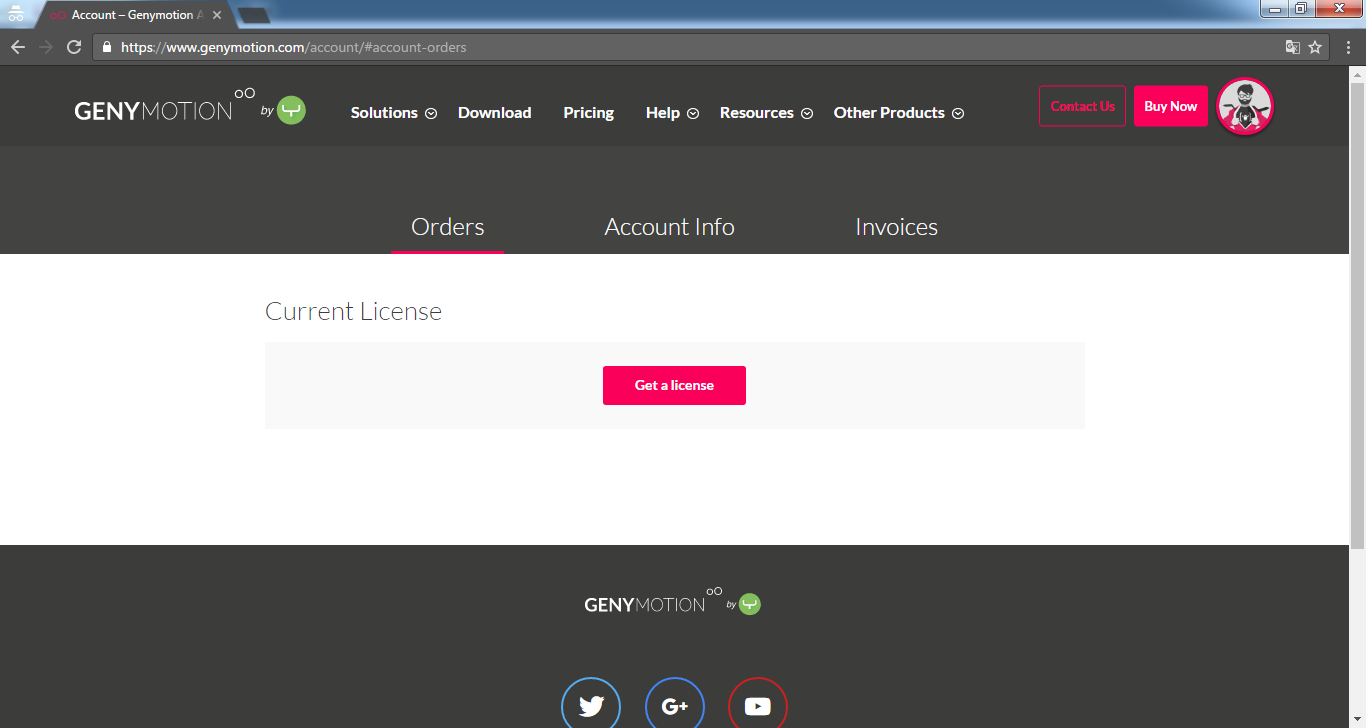
\includegraphics[scale=.35]{setup-genymotion-3}}
							\end{center}
							\caption{Đăng nhập tài khoản trên Genymotion}
							\label{Fig:setup-genymotion-create}
						\end{figure}
					
					\item Chọn thẻ \verb|Download|, được giao diện như hình~\ref{Fig:setup-genymotion-4}: chọn phiên bản \verb|with| \verb|VirtualBox| để tải về máy. Ví dụ như trên hình~\ref{Fig:setup-genymotion-4} tải gói có dung lượng \verb|154MB|.
						\begin{figure}[!h]
							\begin{center}
								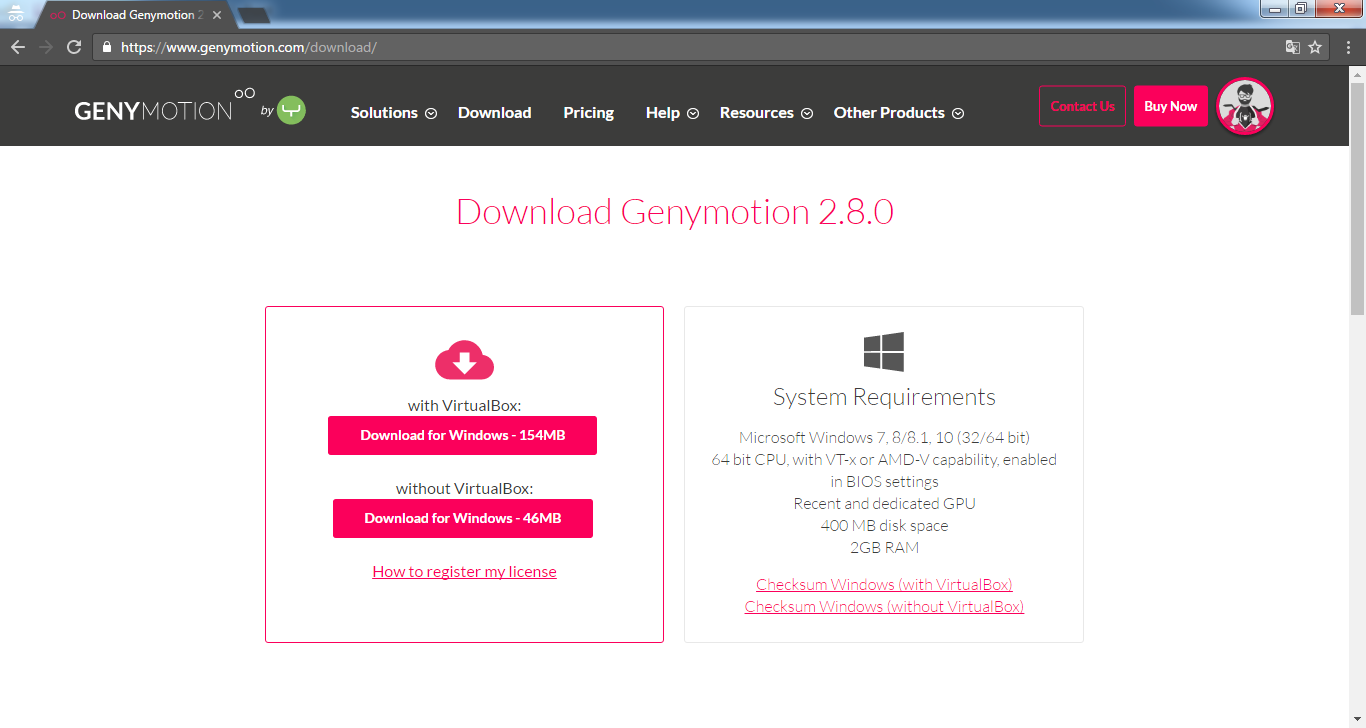
\includegraphics[scale=.35]{setup-genymotion-4}
							\end{center}
							\caption{Download Genymotion về máy}
							\label{Fig:setup-genymotion-4}
							\vspace{-.25cm}
						\end{figure}			
				\end{itemize}
			
			\item \textit{Bước 2:} Cài đặt phần mềm \verb|Genymotion| và \verb|Oracle VM VirtulaBox|.
				\begin{itemize}
					\item Mở phần mềm \verb|Genymotion| vừa tải về, được giao diện như hình~\ref{Fig:setup-genymotion-5}: chọn \verb|Run| để bắt đầu cài đặt.
					
					\item Được giao diện như hình~\ref{Fig:setup-genymotion-6}: chọn ngôn ngữ là \verb|English| và chọn \verb|OK|.
					
					\item Trên giao diện hình~\ref{Fig:setup-genymotion-7}: nơi cài đặt chọn như mặc định, chọn \verb|Next|.

					\item Được giao diện hình~\ref{Fig:setup-genymotion-8}: tiếp tục chọn \verb|Next|.			
						\begin{figure}[!h]
							\begin{center}	
								\subfloat[Chọn Run\label{Fig:setup-genymotion-5}]
									{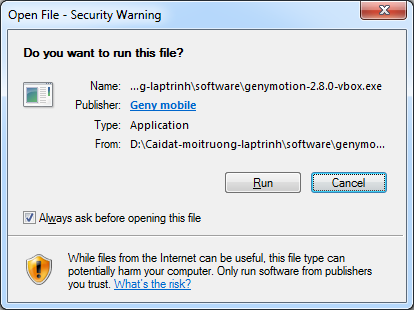
\includegraphics[scale=.6]{setup-genymotion-5}}
								\hspace{.5cm}
								\subfloat[Chọn ngôn ngữ English và chọn OK\label{Fig:setup-genymotion-6}]
									{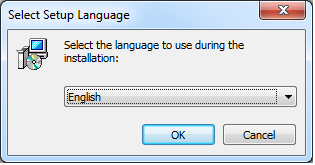
\includegraphics[scale=.75]{setup-genymotion-6}}\\
								\subfloat[Chọn Next\label{Fig:setup-genymotion-7}]
									{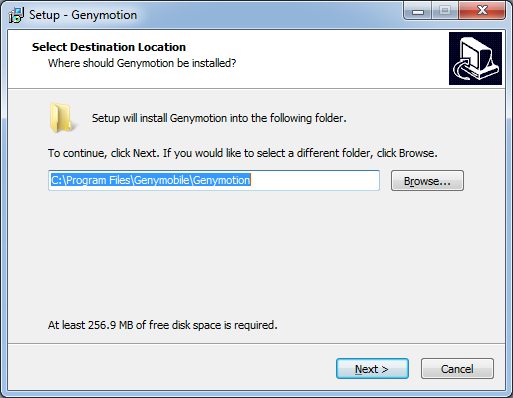
\includegraphics[scale=.5]{setup-genymotion-7}}
								\hspace{.5cm}
								\subfloat[Chọn Next\label{Fig:setup-genymotion-8}]
									{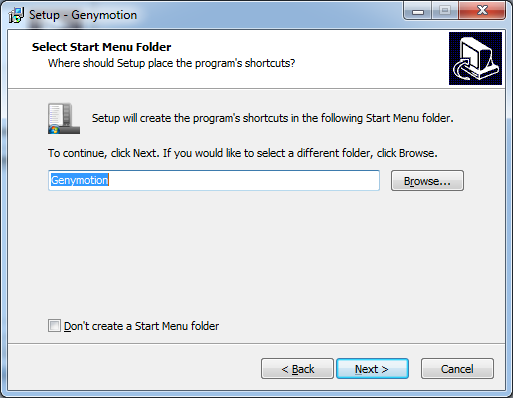
\includegraphics[scale=.5]{setup-genymotion-8}}\\
								\subfloat[Chọn Next\label{Fig:setup-genymotion-9}]
									{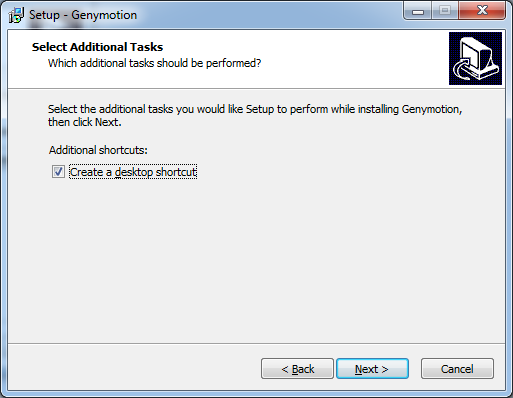
\includegraphics[scale=.5]{setup-genymotion-9}}
								\hspace{.5cm}
								\subfloat[Chọn Install\label{Fig:setup-genymotion-10}]
									{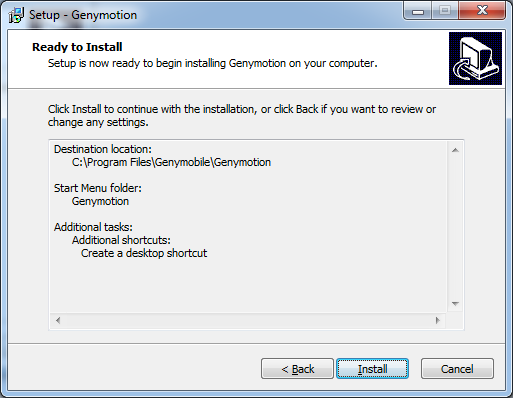
\includegraphics[scale=.5]{setup-genymotion-10}}\\								
							\end{center}
							\vspace{-.25cm}
							\caption{Cài đặt Genymotion trên Windows}
							\label{Fig:setup-genymotion-windows}
							\vspace{-.75cm}
						\end{figure}
						
					\item Đến phần cài đặt \verb|Oracle VM VirtualBox| (được tích hợp sẳn trong gói \verb|Genymotion|), được giao diện như hình~\ref{Fig:setup-genymotion-11}: chọn \verb|Next|.
					
					\item Được giao diện như hình~\ref{Fig:setup-genymotion-12}: để nơi cài đặt như mặc định, chọn \verb|Next|.
					
					\item Được giao diện như hình~\ref{Fig:setup-genymotion-13}: chọn \verb|Next|. Được giao diện như hình~\ref{Fig:setup-genymotion-14}: chọn \verb|Yes|.
					
					\item Được giao diện như hình~\ref{Fig:setup-genymotion-15}: chọn \verb|Install| để cài đặt.
					
					\item Trong quá trình cài đặt, xuất hiện thông báo như hình~\ref{Fig:setup-genymotion-16}: chọn \verb|Always| \verb|trut software from "Oracle Corporation"| và chọn \verb|Install| để cài đặt.
					
						\begin{figure}[!h]
							\begin{center}	
								\subfloat[Chọn Next\label{Fig:setup-genymotion-11}]
									{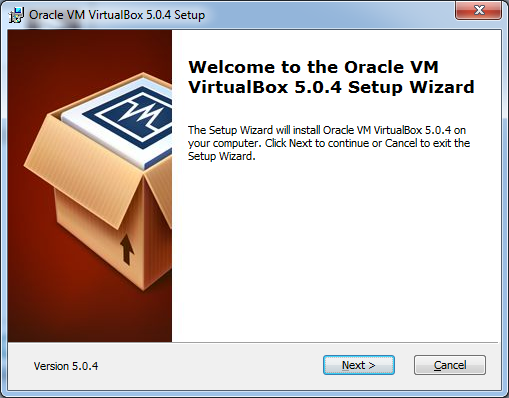
\includegraphics[scale=.5]{setup-genymotion-11}}
								\hspace{.5cm}
								\subfloat[Chọn Next\label{Fig:setup-genymotion-12}]
									{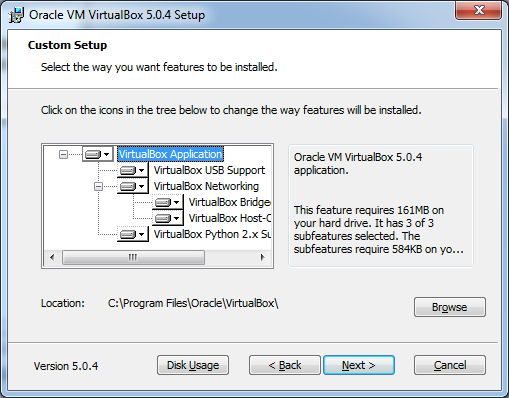
\includegraphics[scale=.5]{setup-genymotion-12}}\\
								\subfloat[Chọn Next\label{Fig:setup-genymotion-13}]
									{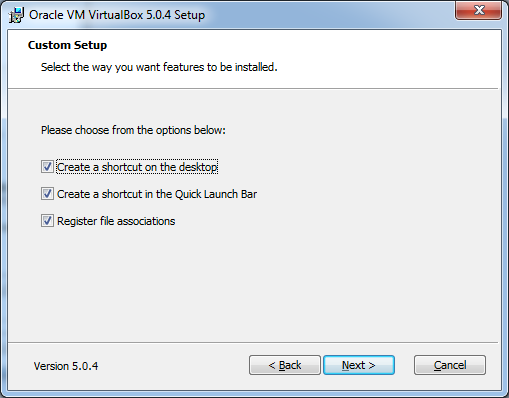
\includegraphics[scale=.5]{setup-genymotion-13}}
								\hspace{.5cm}
								\subfloat[Chọn Yes\label{Fig:setup-genymotion-14}]
									{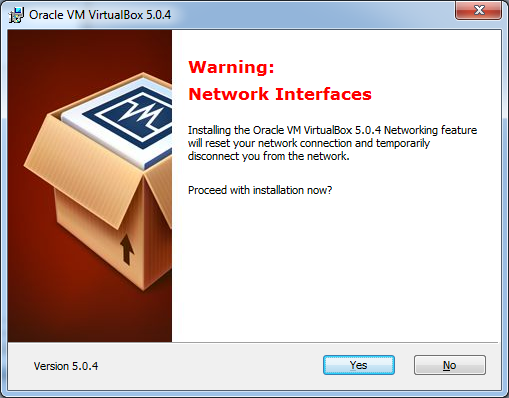
\includegraphics[scale=.5]{setup-genymotion-14}}\\
								\subfloat[Chọn Install\label{Fig:setup-genymotion-15}]
									{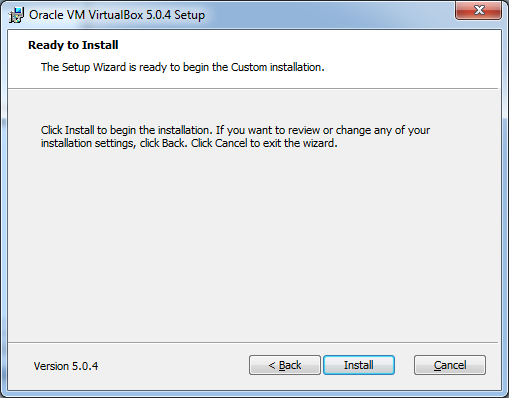
\includegraphics[scale=.5]{setup-genymotion-15}}
								\hspace{.5cm}
								\subfloat[Check chọn  Always trust\ldots và chọn Install\label{Fig:setup-genymotion-16}]
									{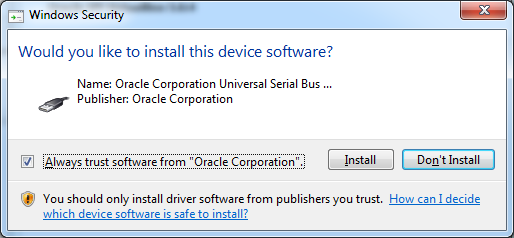
\includegraphics[scale=.5]{setup-genymotion-16}}\\								
							\end{center}
							\vspace{-.25cm}
							\caption{Cài đặt Oracle VM VirtualBox trên Windows}
							\label{Fig:setup-oracle-windows}
							\vspace{-.5cm}
						\end{figure}
						
					\item Quá trình cài đặt \verb|Genymotion| và \verb|Oracle VM VirtualBox| hoàn thành được giao diện như hình~\ref{Fig:setup-oracle-windows-complete}: chọn \verb|Finish| để mở các phần mềm lần đầu tiên để thiết lập.
						\begin{figure}[!h]
							\vspace{-1cm}
							\begin{center}	
								\subfloat[Chọn Finish\label{Fig:setup-genymotion-17}]
									{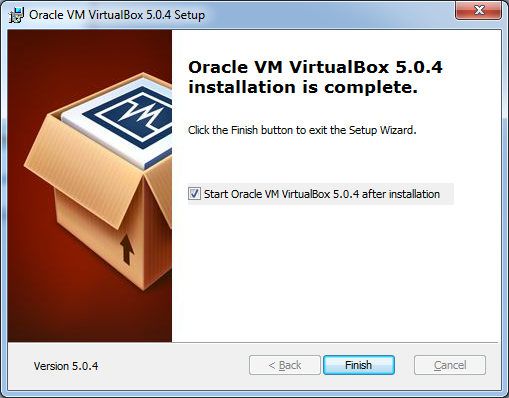
\includegraphics[scale=.5]{setup-genymotion-17}}
								\hspace{.5cm}
								\subfloat[Giao diện của Oracle VM VirtualBox Manager\label{Fig:setup-genymotion-18}]
									{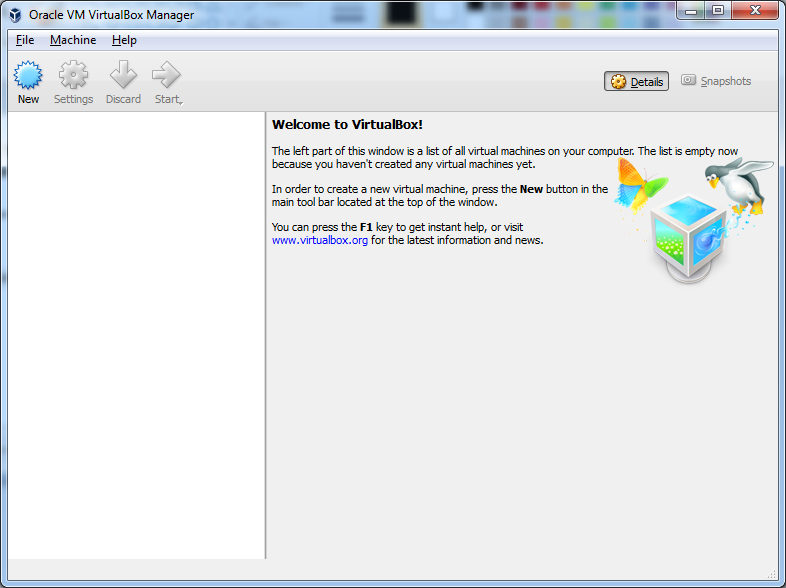
\includegraphics[scale=.34]{setup-genymotion-18}}\\
								\subfloat[Chọn Finish\label{Fig:setup-genymotion-19}]
									{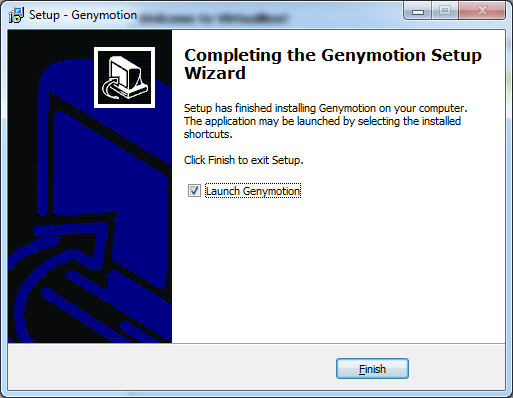
\includegraphics[scale=.5]{setup-genymotion-19}}
								\hspace{2cm}
								\subfloat[Mở Genymotion\label{Fig:setup-genymotion-20}]
									{\includegraphics[scale=.4]{setup-genymotion-20}}\\				
							\end{center}
							\caption{Hoàn thành cài đặt Genymotion và Oracle VM VirtualBox trên Windows}
							\label{Fig:setup-oracle-windows-complete}
						\end{figure}
				\end{itemize}
			\item \textit{Bước 3:} Tải thiết bị ảo trên \verb|Genymotion| về máy để thực hiện mô phỏng.
				\begin{itemize}
					\item Khi mở \verb|Genymotion| lần đầu tiên, xuất hiện thông báo như hình~\ref{Fig:setup-genymotion-21}: chọn \verb|Acept|.
					
					\item Do mới cài đặt nên chưa có thiết bị máy ảo nào được tải về, được giao diện như hình~\ref{Fig:setup-genymotion-22}: chọn \verb|Yes| để tải thiết bị mới về máy.
					
					\item Được giao diện như hình~\ref{Fig:setup-genymotion-23}: chọn \verb|Sign in| để đăng nhập xem tất cả các máy ảo.
					
					\item Xuất hiện thông báo như hình~\ref{Fig:setup-genymotion-24}: nhập vào \verb|Username| và \verb|Password| đã đăng ký lúc tải \verb|Genymotion| từ trang chủ về máy.
					
					\item Sau khi đăng nhập thành công, chúng ta thấy danh sách các thiết bị máy ảo như hình~\ref{Fig:setup-genymotion-25}. Chọn bất kỳ một máy ảo nào đó, ví dụ chọn máy ảo \verb|Google Nexus 4 - 4.3 - API - 768x1280| (hình~\ref{Fig:setup-genymotion-26}), có thông tin máy cho trên hình ~\ref{Fig:setup-genymotion-27}, chọn \verb|Next| để tải máy ảo về máy. Đợi quá trình tải hoàn thành, được giao diện như hình~\ref{Fig:setup-genymotion-28}: chọn \verb|Finish| để hoàn tất.
						\begin{figure}[!h]
							\begin{center}	
								\subfloat[Chọn Acept\label{Fig:setup-genymotion-21}]
									{\includegraphics[scale=.5]{setup-genymotion-21}}
								\hspace{.5cm}
								\subfloat[Chọn Yes\label{Fig:setup-genymotion-22}]
									{\includegraphics[scale=.73]{setup-genymotion-22}}\\
								\subfloat[Chọn Sign in\label{Fig:setup-genymotion-23}]
									{\includegraphics[scale=.3]{setup-genymotion-23}}
								\hspace{.5cm}
								\subfloat[Nhập thông tin đăng nhập\label{Fig:setup-genymotion-24}]
									{\includegraphics[scale=.8]{setup-genymotion-24}}\\
								\subfloat[Danh sách các máy ảo\label{Fig:setup-genymotion-25}]
									{\includegraphics[scale=.3]{setup-genymotion-25}}
								\hspace{.5cm}
								\subfloat[Chọn bất kỳ một máy ảo nào và chọn Next\label{Fig:setup-genymotion-26}]
									{\includegraphics[scale=.3]{setup-genymotion-26}}\\
									
								\subfloat[Xem thông tin máy ảo và chọn Next\label{Fig:setup-genymotion-27}]
									{\includegraphics[scale=.3]{setup-genymotion-27}}
								\hspace{.5cm}
								\subfloat[Quá trình tải máy ảo về máy\label{Fig:setup-genymotion-28}]
									{\includegraphics[scale=.3]{setup-genymotion-28}}\\								
							\end{center}
							\caption{Tải máy ảo Genymotion về máy}
							\label{Fig:download-virtual-devices}
							\vspace{-.5cm}
						\end{figure}
					
					\item Khi tải thiết bị máy ảo thành công, danh sách \verb|Your Virtual Devices| có tên thiết bị vừa tải về như hình~\ref{Fig:setup-genymotion-29}: chọn máy ảo và chọn \verb|Start| để mở máy ảo lên kiểm tra (như hình~\ref{Fig:setup-genymotion-30}), nếu khởi động máy ảo thành công thì được kết quả như hình~\ref{Fig:setup-genymotion-31} và~\ref{Fig:setup-genymotion-32} (tùy thuộc vào cấu hình máy mà quá trình khởi động nhanh hay chậm).
						\begin{figure}[!h]
							\begin{center}	
								\subfloat[Chọn máy ảo và chọn Start\label{Fig:setup-genymotion-29}]
									{\includegraphics[scale=.35]{setup-genymotion-29}}
								\hspace{.5cm}
								\subfloat[Quá trình kiểm tra mở máy ảo\label{Fig:setup-genymotion-30}]
									{\includegraphics[scale=.73]{setup-genymotion-30}}\\
								\subfloat[Quá trình khởi động máy ảo\label{Fig:setup-genymotion-31}]
									{\includegraphics[scale=.5]{setup-genymotion-31}}
								\hspace{1.5cm}
								\subfloat[Khởi động máy ảo thành công\label{Fig:setup-genymotion-32}]
									{\includegraphics[scale=.5]{setup-genymotion-32}}\\			
							\end{center}
							\caption{Mở máy ảo Genymotion để kiểm tra}
							\label{Fig:open-virtual-devices}
							\vspace{-.5cm}
						\end{figure}				
				\end{itemize}
			\item Sau này muốn mở máy ảo lên sử dụng thì chọn \verb|shortcut| có tên là \verb|Genymotion| (không mở \verb|shortcut| có tên \verb|Genymotion Shell| do chưa cần dùng đến), sẽ có giao diện như hình~\ref{Fig:setup-genymotion-29}:
				\begin{itemize}
					\item Muốn khởi động thiết bị thì chọn thiết bị và nhấn vào nút \verb|Start|.
					\item Muốn thêm thiết bị mới thì nhấn vào nút \verb|Add| và chọn thiết bị mới.
				\end{itemize}
		\end{itemize}
%%-------------------------------------------------------------------------------------------------------------------------------------%%
%%-------------------------------------------------------------------------------------------------------------------------------------%%
\chapter{Tìm hiểu OpenGL ES 2.0 trên Android}
\section{Kiểu dữ liệu trong OpenGL ES}
	Với một số lệnh tham số truyền vào là các kiểu dữ liệu được cho trong bảng~\ref{Tab:kieudulieu-opengles}.
	\begin{table}[!h]
		\begin{center}
			\begin{tabular}{|c|l|l|l|}\hline
				\textit{Hậu tố} & \textit{Kiểu dữ liệu} & \textit{Ứng với kiểu trong C} & \textit{Ứng với kiểu trong OpenGL}\\ \hline
				b & 8-bit signed integer & signed char & GLbyte \\ \hline
				ub & 8-bit unsigned integer & unsigned char & GLubyte, GLboolean \\ \hline
				s & 16-bit signed integer & short & GLshort \\ \hline
				us & 16-bit unsigned integer & unsigned short & GLushort \\ \hline
				i & 32-bit signed integer & int & GLint \\ \hline
				ui & 32-bit unsigned integer & unsigned int & GLuint, GLbitfield, GLenum \\ \hline
				x & 16.16 fixed point & int & GLfixed \\ \hline
				f & 32-bit floating point & float & GLfloat, GLclampf \\ \hline
			\end{tabular}
		\end{center}
		\caption{Kiểu dữ liệu trong OpenGL ES}
		\label{Tab:kieudulieu-opengles}
	\end{table}
	
	Phần mô tả các lệnh của OpenGL ES 2.0 cùng với kiểu dữ liệu của tham số được cho trong tài liệu có địa chỉ \url{https://www.khronos.org/opengles/sdk/docs/man/}
\section{Sử dụng OpenGL ES 2.0 trong Android}
Có hai lớp chính để tạo và thực thi đồ họa với OpenGL ES API: \verb|GLSurfaceView| và \verb|GLSurfaceView.Renderer|
	
	\begin{itemize}
		\item \verb|GLSurfaceView|: là View mà chúng ta vẽ, thao tác các đối tượng trên đó.
		
		\item \verb|GLSurfaceView.Renderer|: là một Interface định nghĩa các Methods được yêu cầu để vẽ đồ họa trên \verb|GLSurfaceView|. Chúng ta cần cải tiến các Methods sau:
			\begin{itemize}
				\item \verb|onSurfaceCreated()|: hệ thống gọi phương thức này một lần khi tạo \verb|GLSurfaceView|. Dùng phương thức này để thực hiện những hành động chỉ cần tạo ra một lần như cài đặt tham số môi trường OpenGL hoặc khởi tạo các đối tượng đồ họa OpenGL.
				
				\item \verb|onDrawFrame()|: hệ thống gọi phương thức này khi vẽ lại \verb|GLSurfaceView|.
				
				\item \verb|onSurfaceChanged()|: hệ thống gọi phương thức này khi \verb|GLSurfaceView| thay đổi kích thước.
			\end{itemize}
	\end{itemize}
	
	Để sử dụng OpenGL ES 2.0 yêu cầu Android 2.2 (API Level 8) hoặc cao hơn.
\subsection{Khai báo sử dụng OpenGL ES 2.0 trong file Mainfest}
	Thêm vào file \verb|AndroidMainfest.xml| khai báo sau:	
		\begin{lstlisting}[language=XML]
<uses-feature android:glEsVersion="0x00020000" android:required="true" />
		\end{lstlisting}
	
	\begin{itemize}
		\item Nếu xuất hiện lỗi \verb|Default Activity not found|, khắc phục bằng cách thêm đoạn code bên dưới vào file \verb|AndroidMainfest.xml| (nằm trong thẻ \verb|application|):
		\begin{lstlisting}[language=XML]
<activity
	android:name="name_package.MainActivity"
	android:label="@string/app_name">
	<intent-filter>
		<action android:name="android.intent.action.MAIN" />

		<category android:name="android.intent.category.LAUNCHER" />
	</intent-filter>
</activity>
		\end{lstlisting}
	với \verb|name_package| được thay bằng tên của \verb|package| trong \verb|manifest|. \emph{Ví dụ:} cần khai báo như sau:
	
		\begin{lstlisting}[language=XML]
<activity
	android:name="com.opengles.android.opengles20.MainActivity"
	android:label="@string/app_name">
	<intent-filter>
		<action android:name="android.intent.action.MAIN" />

		<category android:name="android.intent.category.LAUNCHER" />
	</intent-filter>
</activity>
		\end{lstlisting}
	\end{itemize}
		
\subsection{Khởi tạo file Activity khi sử dụng OpenGL ES 2.0}
\label{Sec:MainActivity}
	\begin{itemize}
		\item Nội dụng của file \verb|Activity| như bên dưới (tên file \verb|MainActivity.java|):
			\lstinputlisting[language=Java]{MainActivity-1.java}
				
		\item Với đoạn code trên ta thấy cần tạo lớp \verb|GLSurfaceView| để sử dụng trong lớp \verb|Activity|.
	\end{itemize}

\subsection{Xây dựng lớp GLSurfaceView}
\label{Sec:GLSurfaceView}
	\begin{itemize}
		\item Xây dựng lớp \verb|GLSurfaceView| như bên dưới (tên file \verb|MyGLSurfaceView.java|):
			\lstinputlisting[language=Java]{MyGLSurfaceView-1.java}
	\end{itemize}
	
\subsection{Xây dựng lớp Renderer}
\label{Sec:Renderer}
\begin{itemize}
		\item Xây dựng lớp \verb|Renderer| như bên dưới (tên file \verb|MyGLRenderer.java|).
			\lstinputlisting[language=Java]{MyGLRenderer-1.java}
		
		\item Phương thức \verb|onSurfaceCreated|, \verb|onDrawFrame| và \verb|onSurfaceChanged| được giải thích trước đó.
		
		\item Trong lớp \verb|Renderer|, định nghĩa các phương thức để vẽ lên lớp \verb|GLSurfaceView|.
		
		\item Còn vẽ các đối tượng cụ thể thì tạo ra các lớp riêng lớp riêng biệt cho từng đối tượng rồi khai báo vào lớp \verb|Renderer|.
		
		\item Các thao tác sau này chủ yếu là trên lớp \verb|Renderer| và tạo các lớp định nghĩa cho từng đối tượng cụ thể.
	\end{itemize}

\newpage
\subsection{Nội dung của các file chương trình}
	\begin{itemize}
		\item Nội dung của file \verb|AndroidMainfest.xml|:
			\lstinputlisting[language=XML]{AndroidMainfest.xml}
		
		\item Nội dung của file \verb|MainActivity.java|: mục~\ref{Sec:MainActivity} (trang~\pageref{Sec:MainActivity}).
			%\lstinputlisting[language=Java]{MainActivity-1.java}
		
		\item Nội dung của file \verb|MyGLSurfaceView.java|: mục~\ref{Sec:GLSurfaceView} (trang~\pageref{Sec:GLSurfaceView}).
			%\lstinputlisting[language=Java]{MyGLSurfaceView-1.java}
		
		\item Nội dung của file \verb|MyGLRenderer.java|: mục~\ref{Sec:Renderer} (trang~\pageref{Sec:Renderer}).
			%\lstinputlisting[language=Java]{MyGLRenderer-1.java}

		\item Sau khi biên dịch được kết quả như hình \ref{Fig:opengles-1}.
			\begin{figure}[!h]
				\begin{center}
					\includegraphics[scale=.6]{images/opengles-1.png}
				\end{center}
				\caption{Sử dụng OpenGL ES 2.0 trên Android} \label{Fig:opengles-1}
			\end{figure}			
	\end{itemize}

\newpage	
\section{Vẽ đối tượng hình học cơ bản}
	Để vẽ các đối tượng hình học cơ bản thực hiện theo 2 bước:
		\begin{itemize}
			\item \emph{Bước 1:} Định nghĩa các \verb|shapes|.
			
			\item \emph{Bước 2:} Thực hiện vẽ các \verb|shapes| đã định nghĩa trước đó.
			
			\item[$\ast$] Các đối tượng này được định nghĩa trên một lớp riêng.
		\end{itemize}

\subsection{Định nghĩa đối tượng là một tam giác}
	\begin{itemize}
		\item Mỗi đỉnh của tam giác được xác định bởi tọa độ: \verb|(x, y, z)|.
		\item Đối tượng được định nghĩa như bên dưới (file \verb|Triangle.java|):
			\begin{lstlisting}[language=Java]
public class Triangle {

    private FloatBuffer vertexBuffer;

    // number of coordinates per vertex in this array
    static final int COORDS_PER_VERTEX = 3;
    static float triangleCoords[] = {   // in counterclockwise order:
             0.0f,  0.5f, 0.0f,   // top
            -0.5f, -0.5f, 0.0f,   // bottom left
             0.5f, -0.5f, 0.0f    // bottom right
    };

    // Set color with red, green, blue and alpha (opacity) values
    float color[] = {0.0f, 0.6f, 1.0f, 1.0f};

    public Triangle() {
        // initialize vertex byte buffer for shape coordinates
        
        // (number of coordinate values * 4 bytes per float)
        ByteBuffer bb = ByteBuffer.allocateDirect(triangleCoords.length*4);
        // use the device hardware's native byte order
        bb.order(ByteOrder.nativeOrder());

        // create a floating point buffer from the ByteBuffer
        vertexBuffer = bb.asFloatBuffer();
        // add the coordinates to the FloatBuffer
        vertexBuffer.put(triangleCoords);
        // set the buffer to read the first coordinate
        vertexBuffer.position(0);
    }
}
			\end{lstlisting}
	\end{itemize}
	
\subsection{Vẽ đối tượng là một tam giác}
	\begin{itemize}
		\item Trong lớp \verb|Renderer|, khai báo và định nghĩa thêm các phần sau (bước khởi tạo các \verb|shapes| trong phương thức \verb|onSurfaceCreated|).
			\begin{lstlisting}[language=Java]
public class MyGLRenderer implements GLSurfaceView.Renderer {

    ...
    private Triangle mTriangle;

    public void onSurfaceCreated(GL10 unused, EGLConfig config) {
        ...

        // initialize a triangle
        mTriangle = new Triangle();        
    }
    ...
}
			\end{lstlisting}
		
		\item Thực hiện vẽ các \verb|shapes| đã được định nghĩa trước đó (trong file \verb|Triangle.java|):% và \verb|Square.java|).
			\begin{itemize}
				\item Khai báo các dòng sau trong lớp \verb|Triangle|:
					\begin{lstlisting}[language=Java]
public class Triangle {

    private final String vertexShaderCode =
        "attribute vec4 vPosition;" +
        "void main() {" +
        "  gl_Position = vPosition;" +
        "}";

    private final String fragmentShaderCode =
        "precision mediump float;" +
        "uniform vec4 vColor;" +
        "void main() {" +
        "  gl_FragColor = vColor;" +
        "}";

    ...
}						
					\end{lstlisting}
				
				\item Tạo phương thức \verb|loadShader| trong lớp \verb|Renderer|:
					\begin{lstlisting}[language=Java]
public static int loadShader(int type, String shaderCode){

    // create a vertex shader type (GLES20.GL_VERTEX_SHADER)
    // or a fragment shader type (GLES20.GL_FRAGMENT_SHADER)
    int shader = GLES20.glCreateShader(type);

    // add the source code to the shader and compile it
    GLES20.glShaderSource(shader, shaderCode);
    GLES20.glCompileShader(shader);

    return shader;
}					
					\end{lstlisting}
					
				\item Khai báo thêm các dòng sau trong lớp \verb|Triangle|:
					\begin{lstlisting}[language=Java]
public class Triangle() {
    ...

    private final int mProgram;

    public Triangle() {
        ...

        int vertexShader = MyGLRenderer.loadShader(GLES20.GL_VERTEX_SHADER,
                                        vertexShaderCode);
                                        
        int fragmentShader = MyGLRenderer.loadShader(GLES20.GL_FRAGMENT_SHADER,
                                        fragmentShaderCode);

        // create empty OpenGL ES Program
        mProgram = GLES20.glCreateProgram();

        // add the vertex shader to program
        GLES20.glAttachShader(mProgram, vertexShader);

        // add the fragment shader to program
        GLES20.glAttachShader(mProgram, fragmentShader);

        // creates OpenGL ES program executables
        GLES20.glLinkProgram(mProgram);
    }
}					
					\end{lstlisting}
				\item Tạo phương thức \verb|draw| trong lớp \verb|Triangle| để vẽ các \verb|shapes| đã định nghĩa:
					\begin{lstlisting}[language=Java]
private int mPositionHandle;
private int mColorHandle;

private final int vertexCount = triangleCoords.length / COORDS_PER_VERTEX;
private final int vertexStride = COORDS_PER_VERTEX * 4; // 4 bytes per vertex

public void draw() {
    // Add program to OpenGL ES environment
    GLES20.glUseProgram(mProgram);

    // get handle to vertex shader's vPosition member
    mPositionHandle = GLES20.glGetAttribLocation(mProgram, "vPosition");

    // Enable a handle to the triangle vertices
    GLES20.glEnableVertexAttribArray(mPositionHandle);

    // Prepare the triangle coordinate data
    GLES20.glVertexAttribPointer(mPositionHandle, 
                                 COORDS_PER_VERTEX,
                                 GLES20.GL_FLOAT, false,
                                 vertexStride, vertexBuffer);

    // get handle to fragment shader's vColor member
    mColorHandle = GLES20.glGetUniformLocation(mProgram, "vColor");


    // Set color for drawing the triangle
    GLES20.glUniform4fv(mColorHandle, 1, color, 0);

    // Draw the triangle
    GLES20.glDrawArrays(GLES20.GL_TRIANGLES, 0, vertexCount);

    // Disable vertex array
    GLES20.glDisableVertexAttribArray(mPositionHandle);
}					
					\end{lstlisting}							
			\end{itemize}
		
		\item Nội dung của các file chương trình:
			\begin{itemize}
				\item Nội dung của các file \verb|AndroidMainfest.xml|, \verb|MainActivity.java| và \verb|MyGLSurfaceView.java| không thay đổi.
				\item Nội dung của file \verb|MyGLRenderer.java|:
					\lstinputlisting[language=Java]{MyGLRenderer-2.java}					
				
				\item Nội dung của file \verb|Triangle.java|:
					\lstinputlisting[language=Java]{Triangle.java}
			\end{itemize}

\newpage		
		\item Sau khi biên dịch được kết quả như hình \ref{Fig:opengles-2}.
				\begin{figure}[!h]
					\begin{center}
						\includegraphics[scale=.6]{images/opengles-2.png}
					\end{center}
					\caption{Sử dụng OpenGL ES 2.0 vẽ đối tượng là một tam giác} \label{Fig:opengles-2}
				\end{figure}
	\end{itemize}

\chapter{Kết quả}
\section{Kết quả đạt được}
	Qua quá trình thực hiện niên luận, nhóm chúng em đạt được một số kết quả sau:
		\begin{itemize}
			\item Sử dụng được một số lệnh cơ bản trong thư viện OpenGL ES 2.0 để vẽ các đối tượng cơ bản.
			
			\item Nhúng các mã lệnh của OpenGL vào chương trình Android.
		\end{itemize}
\section{Hạn chế}
	Bên cạnh kết quả đạt được, nhóm chúng em còn gặp một số hạn chế như sau:
		\begin{itemize}
			\item Còn hạn chế về kiến thức đồ họa và các kiến thức toán liên quan đến đồ họa.
			
			\item Chỉ mới sử dụng được OpenGL ở mức độ cơ bản, chưa khai thác được hết các lệnh trong thư viện.		
		\end{itemize}
\section{Hướng phát triển}
Nhóm em có định hướng phát triển đề tài như sau: ``\emph{Xây dựng phần mềm vẽ hình không gian trên điện thoại di động bằng cách sử dụng thư viện OpenGL ES phục vụ mục đích học tập.}''\\

	Ý tưởng xây dựng phần mềm:
	\begin{itemize}
		\item Người vẽ có thể chọn vị trí các đỉnh trong hệ tọa độ rồi nối các đỉnh lại với nhau để tọa thành hình hoàn chỉnh.
		
		\item Sau khi đã vẽ được hình hoàn chỉnh, người vẽ có thể xoay hình theo các hướng để quan sát dễ dàng hơn.	
		
		\item Có thể cắt khối hình ra để quan sát chi tiết bên trong.
		
		\item Giải quyết một số bài toán liên quan đến hình học không gian, phục vụ học tập: tính thể tích, diện tích, tìm tọa độ điểm, phương trình đường thẳng, mặt phẳng,\ldots
		
		\item Giải quyết vấn đề liên quan đến vẽ kỹ thuật:
			\begin{itemize}
				\item Từ một mô hình của vật thể trong không gian được người dùng vẽ lên, thực hiện phép chiếu theo một tiêu chuẩn cụ thể nào đó, thì chương trình sẽ tự động tìm ra được hình chiếu đứng hình, hình chiếu bằng, hình chiếu cạch của vật thể. 
				\item Hoặc ngược lại từ hình chiếu đứng, hình chiếu bằng, hình chiếu cạnh, chương trình có thể tự động vẽ lại được mô hình của vật thể trong không gian.
			\end{itemize}				
	\end{itemize}

\chapter*{Tài liệu tham khảo}
\addcontentsline{toc}{chapter}{\textbf{Tài liệu tham khảo}}
	\begin{enumerate}[{[1]}]
		\item \textbf{Aaftab Munshi -- Dan Ginsburg -- Dave Shreiner}, OpenGL ES 2.0 Programming Guide -- Chapter 1, Pearson Education, Inc., 2009.
		
		\item \href{https://developer.android.com/index.html}{\textbf{Android Developer}}, \href{https://developer.android.com/training/graphics/opengl/index.html}{Displaying Graphics with OpenGL ES}
		
		\href{https://developer.android.com/training/graphics/opengl/index.html}{https://developer.android.com/training/graphics/opengl/index.html} (25/11/2016)
		
		\item \href{ehchua@ntu.edu.sg}{\textbf{Chua Hock-Chuan}}, \href{https://www3.ntu.edu.sg/home/ehchua/programming/android/Android_3D.html#zz-2.3}{Android Programming 3D Graphics with OpenGL ES (Including Nehe's Port)}, \href{https://www3.ntu.edu.sg/home/ehchua/programming/index.html}{Programming notes}
			
			\href{https://www3.ntu.edu.sg/home/ehchua/programming/android/Android_3D.html#zz-2.3}{https://www3.ntu.edu.sg/home/ehchua/programming/android/Android\_3D.html\#zz-2.3}(22/11/2016)		
			
		\item Aksed: \textbf{CoderOfHonor} - Answered: \textbf{Reigertje}, \href{http://stackoverflow.com/questions/17288113/where-is-the-documentation-for-opengl-es-2-0-on-android}{Where is the documentation for OpenGL ES 2.0 on Android?}, \href{http://stackoverflow.com/}{Stackoverflow}.
		
		\href{http://stackoverflow.com/questions/17288113/where-is-the-documentation-for-opengl-es-2-0-on-android}{http://stackoverflow.com/questions/17288113/where-is-the-documentation-for-opengl-es-2-0-on-android} (15/11/2016)
		
		\item \textbf{Hoàng Vũ Nam}, \href{http://blog.rikkeisoft.com/opengl-es-voi-android/}{OpenGL ES với Android}, \href{http://blog.rikkeisoft.com/}{Rikkeisoft Blog}
		
		\href{http://blog.rikkeisoft.com/opengl-es-voi-android/}{http://blog.rikkeisoft.com/opengl-es-voi-android/} (15/11/2016)
		
		\item \textbf{Kevin Brothaler}, OpenGL ES 2 for Android -- A Quick-Start Guide, The Pragmatic Programmers, LLC., 2013.		
		
		\item \textbf{Khoa Phạm}, \href{https://www.youtube.com/watch?v=n1iOKgVhMoM&list=PLzrVYRai0riTlWPxOEhi1-2QmvLiw0DCb}{Lập trình Android cơ bản: Cài đặt Android Studio}, \href{https://www.youtube.com}{Youtube}
		
		\href{https://www.youtube.com/watch?v=n1iOKgVhMoM&list=PLzrVYRai0riTlWPxOEhi1-2QmvLiw0DCb}{https://www.youtube.com/watch?v=n1iOKgVhMoM\&list=PLzrVYRai0riTlWPxOEhi1-2QmvLiw0DCb} (15/11/2016)			

		\item \href{https://www.khronos.org/opengles/sdk/}{\textbf{OpenGL ES Software Development Kit}}, \href{https://www.khronos.org/opengles/sdk/docs/man/}{OpenGL ES 2.0 Reference Pages}.
		
		\href{https://www.khronos.org/opengles/sdk/docs/man/}{https://www.khronos.org/opengles/sdk/docs/man/} (20/11/2016)
							
	\end{enumerate}
\end{document}